%% LyX 2.2.1 created this file.  For more info, see http://www.lyx.org/.
%% Do not edit unless you really know what you are doing.
\documentclass[12pt,a4paper,english,intoc,bibliography=totoc,index=totoc,BCOR10mm,captions=tableheading,titlepage,fleqn]{scrbook}
\usepackage{lmodern}
\renewcommand{\sfdefault}{lmss}
\renewcommand{\ttdefault}{lmtt}
\usepackage[T1]{fontenc}
\usepackage[utf8]{inputenc}
\usepackage{fancyhdr}
\pagestyle{fancy}
\setcounter{secnumdepth}{3}
\setlength{\parskip}{\medskipamount}
\setlength{\parindent}{0pt}
\usepackage{babel}
\usepackage{verbatim}
\usepackage{mathtools}
\usepackage{amsmath}
\usepackage{amssymb}
\usepackage{graphicx}
\usepackage{multirow}
\usepackage{bm}
\usepackage{xcolor}
\usepackage{algpseudocode}
\usepackage{subcaption}
\usepackage{rotating}
\usepackage[ruled,vlined,noresetcount]{algorithm2e}

\SetKwRepeat{Do}{do}{while}
\algnewcommand\algorithmicforeach{\textbf{for each}}
\algdef{S}[FOR]{ForEach}[1]{\algorithmicforeach\ #1\ \algorithmicdo}

\usepackage{CJKutf8}
\newcommand*{\Ja}[1]{%
  \begin{CJK}{UTF8}{ipxg}#1\end{CJK}}

\def\bv #1{\boldsymbol{\mathrm{#1}}}%%%%vector
\def\bm #1{\boldsymbol{#1}}%%%%%matrix
\def\vct#1{\mbox{\boldmath $#1$}}
\def\sub#1{_{\rm #1}}
\newcommand{\argmax}{\mathop{\rm arg~max}\limits}
\newcommand{\argmin}{\mathop{\rm arg~min}\limits}
\newcommand{\newmin}{\mathop{\rm min}\limits}
\newcommand{\newmax}{\mathop{\rm max}\limits}

\newcommand{\onedot}{.\null}
\newcommand{\etal}{\emph{et al}\onedot}
\def\eg{\emph{e.g}\onedot}
\def\ie{\emph{i.e}\onedot}
\def\Eg{\emph{E.g}\onedot}
\def\etal{\emph{et al}\onedot}
\newcommand{\cai}[1]{\textcolor{purple}{[Cai: #1]}}
\DeclareOldFontCommand{\it}{\normalfont\itshape}{\mathit}
\DeclareOldFontCommand{\rm}{\normalfont\rmfamily}{\mathrm}

\PassOptionsToPackage{normalem}{ulem}
\usepackage{ulem}
\usepackage{nomencl}
% the following is useful when we have the old nomencl.sty package
\providecommand{\printnomenclature}{\printglossary}
\providecommand{\makenomenclature}{\makeglossary}
\makenomenclature
\usepackage[unicode=true,pdfusetitle,
 bookmarks=true,bookmarksnumbered=true,bookmarksopen=true,bookmarksopenlevel=1,
 breaklinks=false,pdfborder={0 0 0},pdfborderstyle={},backref=false,colorlinks=false]
 {hyperref}
\hypersetup{
 pdfpagelayout=OneColumn, pdfnewwindow=true, pdfstartview=XYZ, plainpages=false}

\makeatletter

%%%%%%%%%%%%%%%%%%%%%%%%%%%%%% LyX specific LaTeX commands.
\pdfpageheight\paperheight
\pdfpagewidth\paperwidth

\newcommand{\noun}[1]{\textsc{#1}}
%% Because html converters don't know tabularnewline
\providecommand{\tabularnewline}{\\}

\@ifundefined{date}{}{\date{}}
%%%%%%%%%%%%%%%%%%%%%%%%%%%%%% User specified LaTeX commands.
% in case somebody want to have the label "Equation"
%\renewcommand{\eqref}[1]{Equation~(\negthinspace\autoref{#1})}

% that links to image floats jumps to the beginning
% of the float and not to its caption
\usepackage[figure]{hypcap}

% the pages of the TOC is numbered roman
% and a pdf-bookmark for the TOC is added
\let\myTOC\tableofcontents
\renewcommand\tableofcontents{%
  \frontmatter
  \pdfbookmark[1]{\contentsname}{}
  \myTOC
  \mainmatter }

% makes caption labels bold
% for more info about these settings, see
% http://mirrors.ctan.org/macros/latex/contrib/koma-script/doc/scrguien.pdf
\setkomafont{captionlabel}{\bfseries}
\setcapindent{1em}

% enables calculations
\usepackage{calc}

% fancy page header/footer settings
% for more information see section 9 of
% http://www.ctan.org/tex-archive/macros/latex/contrib/fancyhdr/fancyhdr.pdf
\renewcommand{\chaptermark}[1]{\markboth{#1}{#1}}
\renewcommand{\sectionmark}[1]{\markright{\thesection\ #1}}

% increases the bottom float placement fraction
\renewcommand{\bottomfraction}{0.5}

% avoids that floats are placed above its sections
\let\mySection\section\renewcommand{\section}{\suppressfloats[t]\mySection}

% increases link area for cross-references and autoname them
% if you change the document language to e.g. French
% you must change "extrasenglish" to "extrasfrench"
% if you uncomment the following lines, you cannot use the reference version Ref+Text in LyX
%\AtBeginDocument{%
% \renewcommand{\ref}[1]{\autoref{#1}}
%}
%\def\refnamechanges{%
% \renewcommand*{\equationautorefname}[1]{}
% \renewcommand{\sectionautorefname}{sec.\negthinspace}
% \renewcommand{\subsectionautorefname}{sec.\negthinspace}
% \renewcommand{\subsubsectionautorefname}{sec.\negthinspace}
% \renewcommand{\figureautorefname}{Fig.\negthinspace}
% \renewcommand{\tableautorefname}{Tab.\negthinspace}
%}
%\@ifpackageloaded{babel}{\addto\extrasenglish{\refnamechanges}}{\refnamechanges}

\def\eg{{\it e.g.}}
\def\ie{{\it i.e.}}
\def\etal{{\it et al.}}

\makeatother

\begin{document}


\subject{Master's Thesis}
\title{Preference-based Personal Adaptation of Image Classification and Image Retrieval Tasks\vspace{1cm}

\includegraphics[scale=0.7]{thesis/images/japtitle.png}\vspace{1cm}}



\author{Onur Guler\\
Advisor: Professor Yoichi Sato\\
Submission Date: Jan 30th, 2020\vspace{1.5cm}}

\publishers{
\includegraphics[scale=0.15]{images/ut-logo}\\
Department of Information and Communication Engineering Graduate School of Information Science and Technology\\
The University of Tokyo\medskip{}
}

\lowertitleback{\textbf{Advisor}\smallskip{}
\\
Prof. Yoichi Sato}

\maketitle
\lhead{\rightmark}

\rhead[\leftmark]{}

\lfoot[\thepage]{}

\cfoot{}

\rfoot[]{\thepage}

\pagestyle{plain}
\pagenumbering{roman}
\addchap*{Abstract}

Image classification and image retrieval tasks commonly use generic solutions that work for hundreds of class categories. However, an average user often requires only a few class categories whether it is for classifying an image or retrieving the most similar images. For example, a chef may require to distinguish between kitchen equipment whereas a researcher would need class categories such as a computer and lab equipment. Daily routines of the users and their limited surroundings are a huge constraint on their usage. By taking into account the user's requirements, it is possible to obtain a personalized, faster and more memory efficient solution.

For the image classification task, we proposed a novel scheme that users can adaptively and memory-efficiently run a part of a convolutional neural network(CNN) according to their needs without any user-side retraining. Our proposed hierarchical CNN structure can be loaded partially into the user's device to reduce the memory consumption of the system. Our experiments show that the hierarchical CNN is significantly reducing the memory usage per user while maintaining the classification accuracy of the system.

By adopting our idea on image retrieval task, Approximate Nearest Neighbor(ANN) search can be improved by reducing the search space according to the user requirements. Most ANN algorithms assume that the query vectors follow a similar distribution with the searched database. However, users have different interests and environments that strongly affects their usage of the image retrieval system as we have mentioned before. Our experiments show that knowing the required class labels of a user allows us to reduce the area of the search space and improve the search time while maintaining the recall.


\newpage


\tableofcontents

\pagenumbering{arabic}
\listoffigures
\addcontentsline{toc}{chapter}{List of Figures}

\listoftables
\addcontentsline{toc}{chapter}{List of Tables}

\cleardoublepage{}

\pagestyle{plain}

\cleardoublepage{}

\pagestyle{fancy}

\lhead[\chaptername~\thechapter]{\rightmark}

\pagestyle{plain}

\lhead[\chaptername~\thechapter]{\rightmark}

\rhead[\leftmark]{}

\lfoot[\thepage]{}

\cfoot{}

\rfoot[]{\thepage}

\chapter{Introduction}\label{introduction}

\section{Overview}

% \begin{figure}[ht]
%     \centering
%     \includegraphics[width=1.0\linewidth]{images/concept-compressed.pdf}
%     \caption[Discovering Objects of Joint Attention]{\textbf{Discovering Objects of Joint Attention}. Joint attention between persons (1) and (2) is detected (highlighted in red boundaries) from first-person videos recorded with points of gaze data (green circles in the video frames.)}
%     \label{fig:concept}
% \end{figure}

% \begin{figure}[t]
%     \centering
%     \includegraphics[width=\linewidth]{images/challenges-compressed.pdf}
%     \caption[Challenges of discovering Objects of Joint Attention]{\textbf{Challenges of discovering Objects of Joint Attention}.}
%     \label{fig:challenges}
% \end{figure}

% \emph{first-person points-of-view videos}
% \footnote{https://www.tobiipro.com/product-listing/tobii-pro-glasses-2/}
% ~\cite{charman1997infants}
% \ref{fig:challenges}

% \begin{itemize}
%     \item Firstly,
%     \item Secondly, 
%     \item Thirdly,
% \end{itemize}

% \section{Challenges and Contributions\label{sec:The-next-section}}

The influence of wearable technology on our lives is gradually getting stronger and becoming part of our lives. 
Image classification and image retrieval systems are widely used on smart phones or other wearable devices.
As the personal usage of these systems are becoming more and more popular, the need for faster and more efficient architectures is highly crucial.

These systems are commonly implemented with multi-purpose functionality to satisfy a wide range of users. 
However, people's surroundings, their employment, their hobbies and interests and various other things affect their usage of these systems 
and they differ from user to user.
Some users may want to recognize a certain breed of an animal 
whereas another user may require to distinguish between kitchen utensils.

We propose a novel solution for both image classification and image retrieval tasks 
that makes use of user requirements to make the systems more efficient and faster while maintaining the accuracy.
Solutions for each task will be introduced in their corresponding sections.



\section{Image Classification}
\label{sec:intro}

In the recent years, convolutional neural networks (CNNs) have become widely used in many areas including personal use. 
Individual uses are supported by service providers who make use of the high-performance computers. 
Service providers train and deploy deep neural network models and 
users download and use the trained models for their specific purposes.

On the one hand, service providers often train a very deep model with high-performance computers to achieve accurate and multi-purpose recognition. 
On the other hand, end-users may have to run the models with a more limited computational resources, e.g., smartphones and wearable devices. 
Moreover, the users do not always require the whole multi-purpose recognition capabilities. 
For instance, they may only need to distinguish a couple of objects they interact with everyday, out of the 1000 diverse classes that can be recognized by training from ImageNet\cite{deng2009imagenet}.

One straightforward idea to mitigate this gap between service providers and users is 
to compress the model based on each individual user's requirements and 
distribute the personally compressed models to the corresponding users. However, it is infeasible to compress the models for every combination of classes and satisfy every single user. 

A solution to above mentioned method would be to ask the users to compress models based on their needs to make it executable with their computational resources and memories and also simple enough for their purposes. 
However, much relevant work requires re-training of the models at user side, 
such as model distillation and pruning, 
which is not always possible given the limited computational power users have.

\begin{figure}
    \centering
    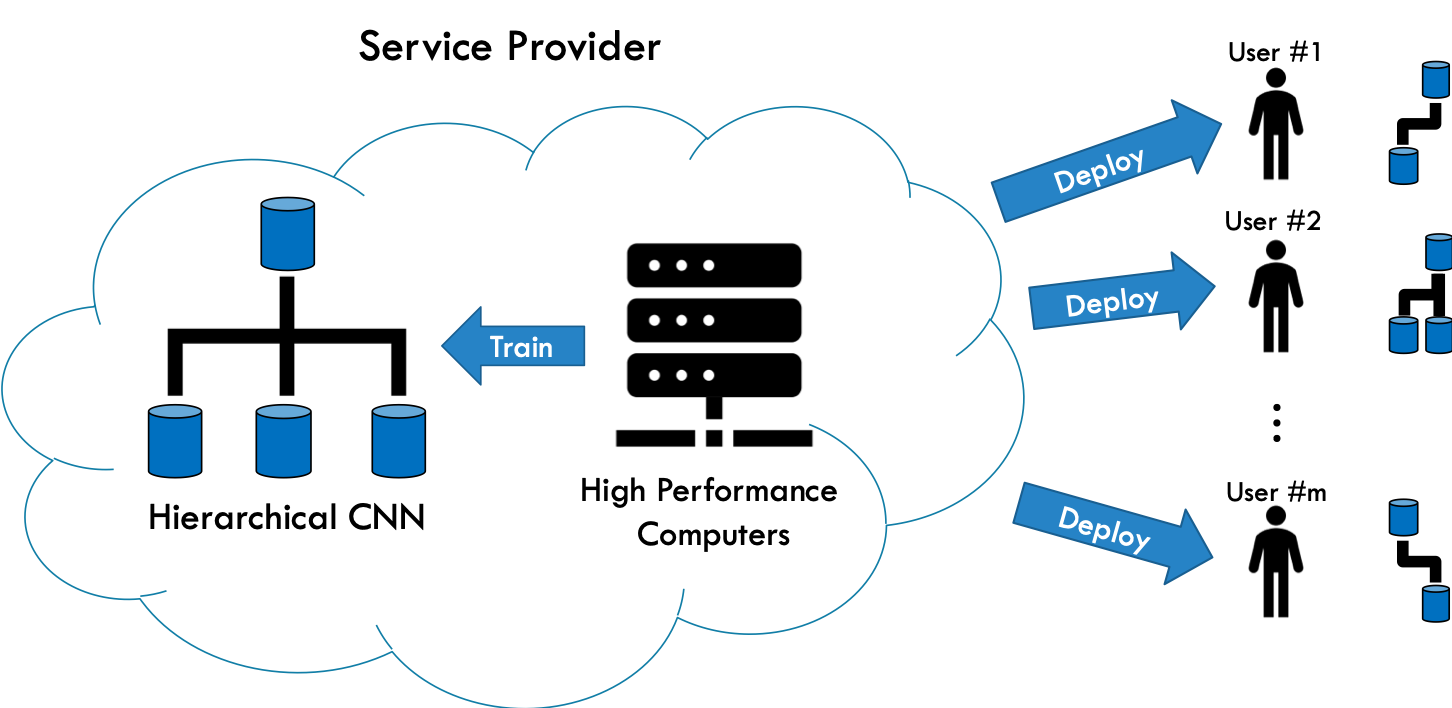
\includegraphics[width=.7\textwidth]{images/ArchitectureOverview(ver2).png}
    \caption{Overview of our scenario-based solution}
    \label{fig:overview}
\end{figure}

We propose a new training strategy that 
allows the users to use a limited part of the trained model based on the classes they encounter in their surroundings. 
The key idea is that the users with different requirements make use of a partially executable model that is trained on service provider side with high computational resources.
This adaptive use allows users to obtain personal simpler models that can run on their devices 
that are limited in memory and computational power without the necessity of re-training the obtained model. 

More specifically, our solution works as in figure \ref{fig:overview}. 
Service providers train a hierarchical
general-purpose network with recognition capabilities of all the possible classes 
that is separable to sub-parts that each recognizes a subset of the classes. 
End-users download and use the part of the network that includes their required subset of the classes.
In this way, each user obtains a smaller model that is tailored for their individual needs.

Additionally, if the users encounter a class that is not in their model, 
the proposed system has the functionality to detect the irregular class and 
downloads extra parts from the full model on the service provider side. 
Thus, the users have access to all the functionality of the complete model if they require.

To evaluate our solution in a scenario-based fashion, 
in our experiments we assume that 
each user encounters a random subset of classes much more likely than 
the rest of the classes due to the limitation of their surroundings. 
Therefore, we tested our approach on generated realistic test users with a biased probability of encountering a subset of classes.

Our hierarchical CNN model is based on a backbone neural network architecture, namely we used VGG16~\cite{simonyan2014very} and MobileNet~\cite{howard2017mobilenets}. 
We compared our solution, hierarchical tree-shaped CNN with \textit{N} branches, with baseline methods for both accuracy and average storage cost for each user. 
We considered two baseline methods, the first one is the backbone CNN that recognize all possible classes 
whereas the second one is \textit{N} smaller models each recognizing a subset of classes.
The latter method differs from our method in the sense that the models do not share any parameters. 
Lastly, we worked with CIFAR-10 and Places365 dataset to compare our method with the baseline methods.


\section{Image Retrieval}

With the advent of internet, everybody had access to enormous amount of digital image data. 
Searching through this big data has become very important. 
Image retrieval is widely used in many applications 
in which there is a image search functionality. 
In this work, we mainly focus on content-based image retrieval (CBIR)
where the content of the image itself is used to search
as opposed to using meta-data or descriptive data of an image.

In image retrieval task, the images are represented with a vector.
Then the task is to find the closest vector to a query vector in a predefined search space. 
Because brute-force searching takes a lot of time, many methods use Approximate Nearest Neighbor (ANN) search for efficiency. 
In ANN algorithms, the search space is divided into sub-spaces. 
When a query vector comes, firstly a few sub-spaces are selected with a high likelihood of containing the true result, 
then only the vectors in those sub-spaces are searched.
Therefore, the search speed is faster with a high probability of finding the true result.

Query vectors are usually assumed to have the same distribution with the searched database. 
However, query images of each user are restricted to user's interests, occupations and mostly their surroundings.
For example in a similar scene image search, a pilot and a police officer would have completely different query images.
Given the different query distribution of each user, it is possible to personalize their search to make it faster.

Our idea is to reduce the search space according to the user requirements to speed up the search. 
Provided that most of the query images are coming from only a part of the search space, the ANN search can be done in that limited space. 
In our experiments, we show that the search becomes faster with a small or no decrease in accuracy.

In our method, we use the classification labels of the images to learn the user requirements. 
We use places365~\cite{zhou2017places} dataset images to construct the search database and the class label information to realize user requirements.
Supposing that the most query images of the users are classified into a number of labels, we can reduce the search space by eliminating sub-spaces not containing those labels.
Then ANN search can be performed in the remaining sub-spaces.


\section{Thesis Outline}

The rest of the thesis is organized as follows. 
In chapter \ref{related}, related work of image classification and image retrieval part will be explained in their respective sections. In chapter \ref{method}, section \ref{sec:HierCNN} will introduce our proposed method on Image classification. 
Details of constructing the hierarchy, obtaining CNN model from the hierarchy, generating realistic users and the baseline of our work will be given. 
Following section \ref{sec:FasterANN} will talk about the method of obtaining vector representation of images, reducing the search space with our proposed method and the baseline in detail.
In Chapter \ref{experiments}, experiments will be shared for each task and the results will be discussed and analyzed in chapter \ref{discussion}. Finally, in chapter \ref{conclusion}, future work will be mentioned along with the conclusive remarks.




\lhead[\chaptername~\thechapter]{\rightmark}

\rhead[\leftmark]{}

\lfoot[\thepage]{}

\cfoot{}

\rfoot[]{\thepage}

\chapter{Related Work}
\label{related}

% Rother \emph{et al.}

Since our idea of using diverse user requirements to personalize the systems for efficiency is applied to both image classification and image retrieval tasks, related work of both tasks will be provided in their respective sections.

\section{Image Classification}

Our proposed method is to obtain a CNN model that can be used partially by each user according to their requirements to be able to distribute efficient models to each user.
As our proposed method aims for efficiency, efficient CNNs will be the main topic in this section.
In the following subsections, efficient CNN models such as various compression methods will be mentioned.
More emphasis will be done to dynamic compression methods.
Moreover, our proposed method is using a hierarchical approach to solve the problem. 
Because of this, we will also address some hierarchical systems that are similar to our proposed model.

\subsection*{Efficient CNNs}

Deep neural network compression techniques reduce the size of the neural networks for a considerable amount. 
There has been much research about how to efficiently compress neural networks, examples of such methods include pruning, parameter sharing(quantization), knowledge distillation etc. 
Generally, compression methods prioritize either memory, computation or energy cost while obtaining more efficient CNN models.

\begin{figure}
    \centering
    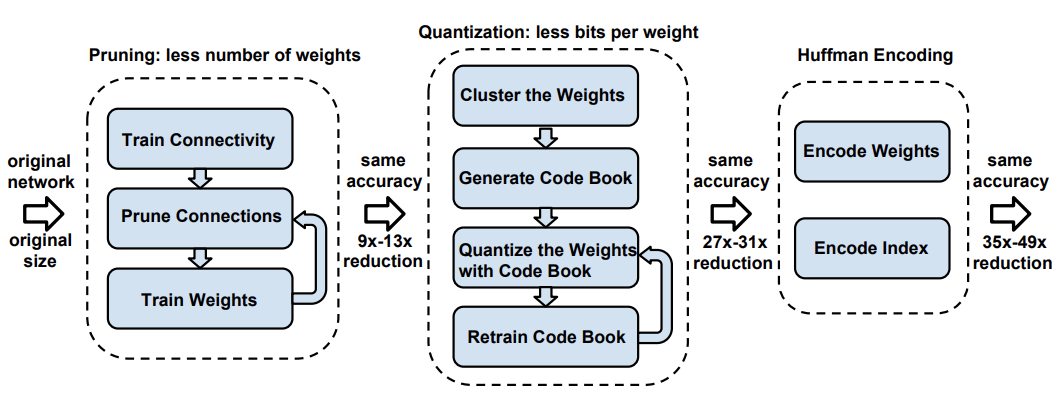
\includegraphics[width=\textwidth]{thesis/images/deep_comp-fig.png}
    \caption{Three steps of Deep Compression by Han et al.\cite{han2015deep}}
    \label{fig:deepcomp}
\end{figure}

Pruning CNN models involves eliminating some individual connections~\cite{molchanov2016pruning} \cite{Yu_2018_CVPR}\cite{Wang2018StructuredPP} or discarding entire channels \cite{He_2017_ICCV}\cite{li2016pruning} that are identified as having a small importance on the output result.
In a famous work about pruning\cite{han2015deep}, Han \emph{et al.} succeeded to reduce the size of VGG-16 by 49x with a 3-step method, as in figure \ref{fig:deepcomp}. 
First step is to prune or eliminate the model connections whose weights are below a threshold. 
In this step, the remaining connections are need to be re-trained for a couple of epochs to maintain the accuracy.
The next step is quantization by grouping the remaining weights into shared weights to reduce the bits to represent the all of the weights.
Last step is using Huffman coding to further reduce the bit representation of all the weights. 
Another way of reducing the model size is knowledge distillation. 
One highly influential example is the work by Hinton \emph{et al.}, where the main idea is to use the output of a large model or an ensemble of specialist models to train a compact network while retaining the accuracy.
Instead of training from the data with definite one-hot coded labels, a larger model is imitated by training a smaller one with the probabilistic outputs of the large model.
In this way, a larger model is condensed into a smaller version.

Not only all the above-mentioned methods require a costly re-training phase to maintain the accuracy,
but also they reduce the size of the model in general, not with respect to each user's requirements of using the model. 
Moreover, our method is to allow users to adaptively use part of the functionality of a model instead of a compression technique.
Having said that, our method can be used jointly with the mentioned works for further reducing the size of the models according to user requirements.

More dynamic approaches include pruning convolutional channels at runtime depending on the input image supported by a RNN network to decide which channels to be omitted~\cite{Lin2017RuntimeNP}. 
As in the figure \ref{fig:runtimenp}, some feature maps are being omitted according to the input image and previously omitted feature maps supervised by RNN.
This method preserves the full ability of the network and improves the speed of the network while maintaining the accuracy. 
The network runs adaptively according to the input images and
can be even fine-tuned for user-requirements to satisfy each user separately.
However, the model is not getting smaller in storage size. 
As one of our concern is the restricted storage memory of wearable devices, it does not serve our purpose of providing users with smaller models custom-made for their requirements. 

Another method, namely AdaDeep~\cite{Liu2018OnDemandDM}, automatically selects a combination of compression techniques especially for deploying neural networks on resource-constrained mobile platforms. 
AdaDeep aims to compress CNN models according to user specifications such as memory limitation, desired accuracy, etc. 
It chooses the best combination of compression algorithms among many different algorithms that prioritize different aspects according to user-specified performance goals and resource constraints. 
Despite serving each user personalized compression, this method is not for adaptively using a sub-functionality of the model.
The resulting model has all the classification functionality that the user does not need for their usage purposes. 
Even though this method satisfies each user's system requirements, it is not removing the undesired functionality of the system to reduce the network size.

\begin{figure}
    \centering
    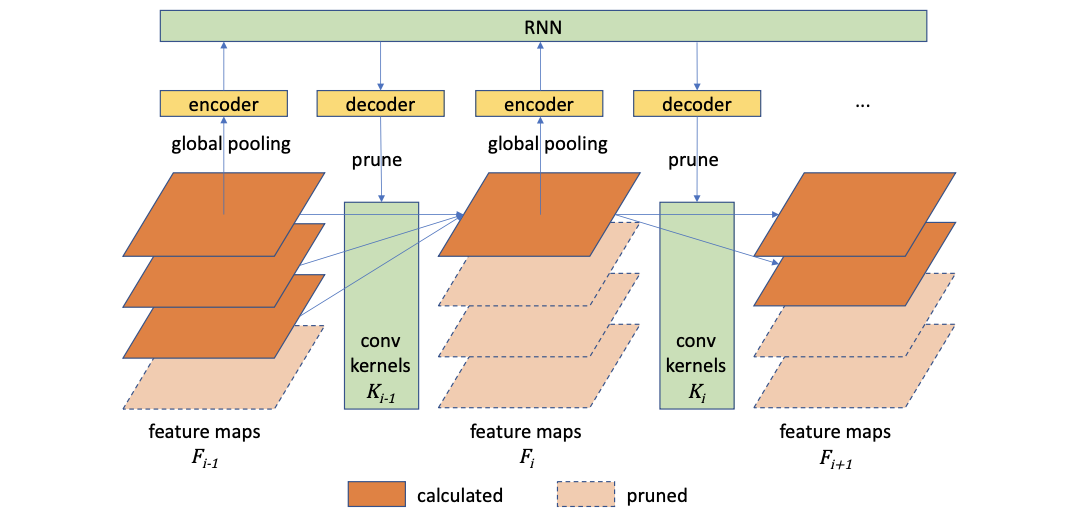
\includegraphics[width=\textwidth]{thesis/images/runtimenp-fig.png}
    \caption{Overall framework of Runtime Neural Pruning\cite{Lin2017RuntimeNP}}
    \label{fig:runtimenp}
\end{figure}

\subsection*{Hierarchical Solutions}

There is plenty of work adopting hierarchically structured CNNs. Roy et al.~\cite{roy2018tree} uses a Tree-CNN to propose a solution for incremental learning. 
In their architecture, the branches of the network grows as new classes added to the model without having an effect on the already learned classes. 
This hierarchical model is similar to our proposed model in this paper, regardless of the problem that it solves. 
HD-CNN~\cite{Yan_2015_ICCV} approaches image classification with the idea that some classes are easy to classify and they only need coarse networks while others require deeper and more complicated networks. 
They make use of a hierarchical classifier to classify easy and hard images on different levels to improve the accuracy. 
Even though, there are various usage of hierarchical CNNs, we believe it is a novel approach to exploit them for allowing users to adaptively use sub-parts of the model according to their individual requirements.

There was one more really similar one I think........

\section{Image Retrieval}

The aim of image retrieval task is to find the closest vector to a query image in a search database, where images are represented by descriptor vectors.
Because the cost of finding the nearest vector is high with traditional algorithms, Approximate Nearest Neighbor (ANN) search is being used for many practical applications.
Our proposed method is built on ANN algorithm to further reduce the area of search space according to user requirements. 
In the following subsections, firstly, various ways of obtaining descriptor vectors from the images will be mentioned. 
Then, recent fast and efficient ANN algorithms will be discussed thoroughly. 

\subsection{Obtaining Descriptors}

Before the arrival of neural networks, SIFT features were mainly used to obtain descriptor vector for the images~\cite{philbin2007object}\cite{jegou2010aggregating}. 
However, CNN-based descriptors quickly substituted the traditional methods. 
Zheng \emph{et al.} compared the performance of many SIFT-based and CNN-based methods on various datasets and superiority of CNN-based methods can clearly be seen. 
Conventional CNN-based methods use a pre-trained model and they take the output of one of the last fully connected layers as the descriptor vector. 
In \cite{babenko2014neural}, they compare the descriptor vectors obtained by the output of different last layers of CNN to see which layer is the best for descriptors.
It is also shown that training the CNN for classification task on a different dataset such as ImageNet gives fairly good results, while fine-tuning the model on the retrieval dataset gives better results.
Later works use only convolutional layers with a following global pooling operation~\cite{razavian2016visual}\cite{tolias2015particular}. 
In a recent state-of-the-art paper for deep global image descriptor~\cite{radenovic2018fine}, descriptor vectors are obtained with convolutional layers followed by a generalized mean pooling operation.

When obtaining descriptor vectors, one should consider the curse of dimensionality. 
As the dimensions of the output layer of CNN can be quite large, most recent works apply whitening with principal component analysis. 
In \cite{jegou2012negative}, whitening is proved to be beneficial and actually improve the accuracy of the retrieval task.

In our work, we simply used VGG-16~\cite{simonyan2014very} pre-trained on ImageNet with the last fully connected layer removed to obtain descriptor vectors. PCA whitening is also applied to reduce the dimension to 64.

\subsection{Approximate Nearest Neighbor Search}

\subsubsection*{Hashing-based methods}

Generally in hashing methods, all database vectors and the query vectors are mapped to lower dimension vectors called \emph{hash-codes} by using several hash functions and the actual search depends on the method. 
In the methods using hash tables and inverted lists, such as Locality Sensitive Hashing (LSH)~\cite{indyk1998approximate}, every hash table has inverted lists on their indices containing the database vectors that falls into one of the lists when the hash function is applied.
Then, only the vectors that are mapped to the same code as the query vector are searched, therefore only a few inverted lists are checked.
On the other hand, other methods compare hash-codes of query and database vectors directly to find the nearest vector.
However, these methods were highly sensitive to data distribution as hash functions should be carefully chosen according to the data. 
As a result, learning-based hashing methods are appeared~\cite{weiss2009spectral}\cite{liu2012supervised}.
There are many different hashing methods based on LSH, varying by the distance or similarity calculation.

\subsubsection*{Quantization-based methods}
\label{subsec:related-quantization}

\begin{figure}
    \centering
    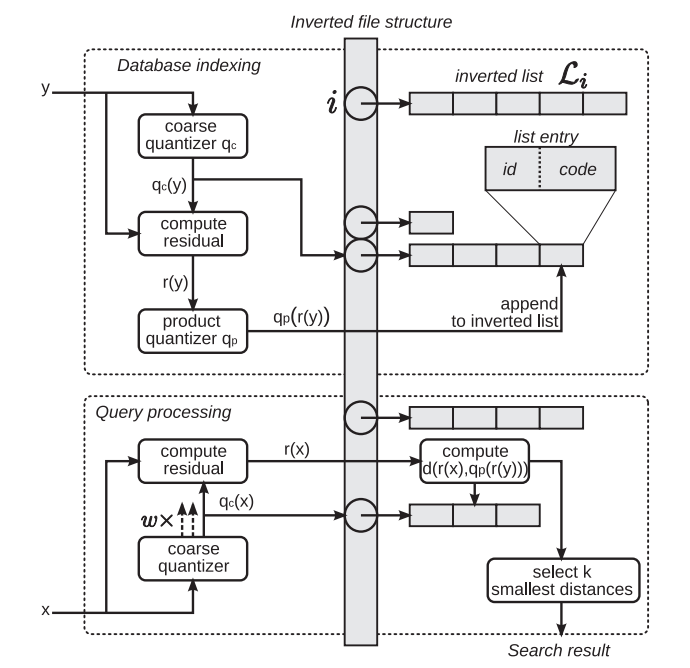
\includegraphics[width=.6\textwidth]{thesis/images/pq-fig.png}
    \caption{Inverted list scheme of Product Quantization\cite{jegou2010product}}
    \label{fig:pq}
\end{figure}

LSH-based methods were outperformed by quantization-based methods, especially for larger-scale data due to their huge memory cost.
In Product Quantization (PQ)~\cite{jegou2010product}, vectors are again mapped to lower dimension vectors to reduce memory consumption. 
However, the number of possible distances, hence the accuracy, is much higher than LSH-based methods using Hamming distance~\cite{weiss2009spectral}.
Moreover, the distances between vectors and the short codes can be calculated fast and accurately.
An inverted list structure, as in figure \ref{fig:pq}, is used to limit the comparison with only the most relevant vectors.

In PQ, search space (database) is divided by using k-means clustering and each quantized database vector are assigned to their respective clusters using euclidian distance. 
Note that, short-coded database vectors are stored with their distance to their respective cluster centroids in their inverted lists, so that the distance can be used to efficiently calculate the closest short code to the query vector.
Quantization of the vectors works as follows.
The vector with dimension $D$ is split into $m$ sub-vectors with same smaller dimensions, $D/m$, and each sub-vector is quantized with different quantizers according to the codebook. 
This quantization scheme reduce the size of the vectors for a great amount.
The search is performed between the query vector and quantized vectors, called Asymmetric Distance Calculation (ADC) instead of quantized query vector and quantized database vectors because Jegou \emph{et al.} showed estimated distances with ADC overlaps more with the true distances.
After finding the closest centroid to the query vector, its distance to the centroid is compared with the distances of the database vectors belonging to that centroid. 
The smallest difference between the distances gives the closest vector.

There are several works that improved product quantization. Optimized Product Quantization (OPQ)\cite{ge2013optimized} changes the problem into an minimization problem of quantization error(lost information with quantization) and optimize codebooks to improve accuracy of PQ with more computational cost. 
On the other hand, Composite Quantization (CQ)\cite{wang2018composite} uses composition of $m$ elements to represent a vector instead of splitting the vector to $m$ equal parts. 
Sub-codewords are added instead to reconstruct the vector. 
Reconstruction error and accuracy is better than that of PQ with additional computational cost.

In our work, we used PQ with inverted list as a baseline for approximate nearest neighbor search. 
We specifically improved the first part of the search where the query vector is compared with the centroids by reducing the number of centroids to check with respect to the user requirements. 

\subsubsection*{Graph-based methods}

\begin{figure}
    \centering
    \begin{subfigure}[b]{0.4\textwidth}
        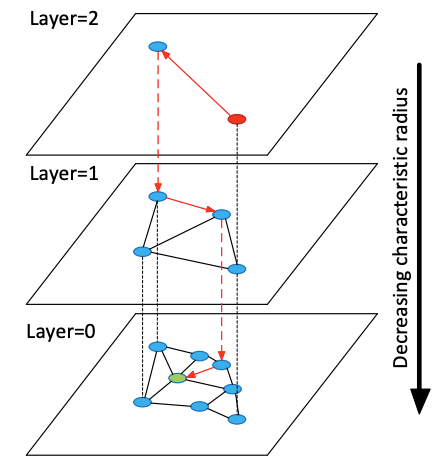
\includegraphics[width=\textwidth]{thesis/images/hnsw-fig.png}
        \caption{The search starts from the top layer with longer connections and continues to lower layers when a local minimum is found.}
        \label{fig:hnsw1}
    \end{subfigure}
  %
    \begin{subfigure}[b]{0.45\textwidth}
        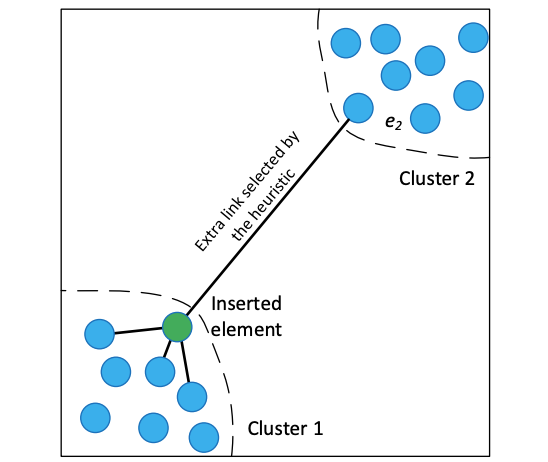
\includegraphics[width=\textwidth]{thesis/images/hnsw-fig2.png}
        \caption{Heuristic chooses an element from another cluster, if inserted element is the closest to $e_2$ compared to other nodes in Cluster 1.}
        \label{fig:hnsw2}
    \end{subfigure}
    \caption{Hierarchical Navigable Small World~\cite{malkov2018efficient}}
    \label{fig:hnsw}
\end{figure}

In graph-based methods, search space is represented with a graph, where the nodes are the database vectors. 
Graph is traversed in a greedy manner to find the closest node to the query vector.
As the database vectors are added to the graph, each node is connected to a few neighboring nodes.
At the beginning of constructing the graph, edges between the few starting nodes are expected to be longer because the probability of finding smaller nodes to connect is higher near the end of construction.
These longer edges are important for fast efficient search.
State-of-the-art work on approximate nearest neighbor search uses an improved version of a graph, namely hierarchical navigable small world (HNSW)\cite{malkov2018efficient}. 
Other NSW methods all suffer from search complexity and scalability. 
HNSW solves the issue by separating the graph into different layers according to the length of the links between the nodes as in figure \ref{fig:hnsw1}. 
Thus, only a fixed number of connections needs to be evaluated for each step because of the hierarchy, which results in a better scalability.
They proposed starting the search from the layer with the longest links to not be stuck in a false local minima. 
The greedy search starts from the upper layers with longer links and continues iteratively towards the lower layers with shorter links when a local minimum is reached.
One other strategy to maintain global connectivity is to add connections between separated clusters with an advanced heuristic\ref{fig:hnsw2}. 
While adding a node to the graph, instead of just connecting the nearest neighbors, an extra link is created to a node in another cluster to improve graph connectivity, therefore improving the probability of traversing until the closest node.




\lhead[\chaptername~\thechapter]{\rightmark}

\rhead[\leftmark]{}

\lfoot[\thepage]{}

\cfoot{}

\rfoot[]{\thepage}

\chapter{Hierarchical CNN}
\label{HierCNN}

\begin{figure}
    \centering
    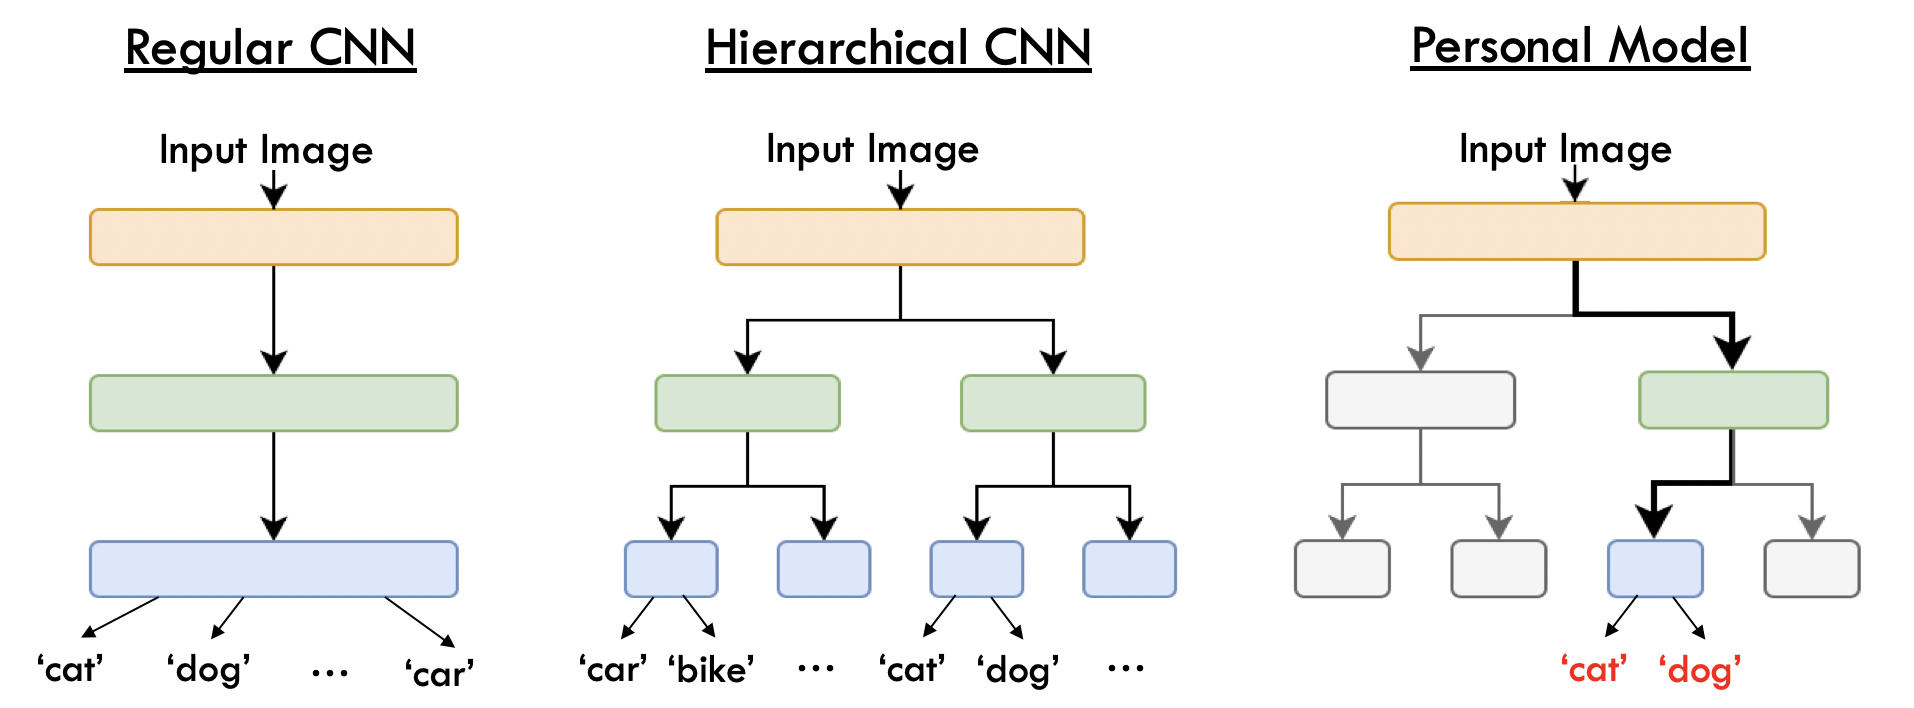
\includegraphics[width=\textwidth]{thesis/images/hierarchical-cnn-fig.png}
    \caption{Regular CNN model on the left is converted to a hierarchical CNN. Users can use only some branches depending on their needs.}
    \label{fig:hiermethodoverview}
\end{figure}

Given a regular CNN model that can recognize many class categories, our method designs a hierarchical CNN which can be used partially according to each user's requirements. 
As it can be seen in the figure \ref{fig:hiermethodoverview}, users are able to use only a single branch of the hierarchical model if they only require a few categories, such as cats and dogs in this case. 
In this way, our method is trying to achieve smaller, memory efficient CNN models that are adapted to each user's personal usages.

There are two steps in our method: creating a hierarchical representation of class categories and building CNN model according to the hierarchy.
In the following subsections, firstly our method will be explained in detail.
Secondly, we explain the process of building the hierarchy and CNN model. 
Then, the details of generating realistic training and test users are shared.
Lastly, we define the baselines to compare with our method.

\section{Method}

In a traditional classification task, a classification model $M$ takes an image $\mathbf{I}$ and generates an output $y\in\mathcal{C}$ with $\mathcal{C} = \{1,2,\dots,C\}$ where $C$ is number of different classes in a dataset. Our goal is to reduce the size of the model $M$. In the following paragraphs, 

User requirements are represented for the each user as $\mathcal{U} \subseteq \mathcal{C}$. 
Given a user requirement $\mathcal{U}$, we want to obtain $M_u$ where $M_u(\mathbf{I}) = c$ and $c\in\mathcal{U}$. 
More importantly, we expect $M_u$ to be smaller than $M$ size, therefore more memory efficient. 
However, traditional CNN models are not separable to smaller models.

Our method builds a hierarchical CNN so that each user can use only a few required branches according to their required labels. 
According to the figure \ref{fig:hiermethodoverview}, the left model $M$ is converted to the hierarchical model. 
Given the user requirements $\mathcal{U}$ as the labels of "cat" and "dog", only the highlighted branch at the right, $M_u$, is loaded into the user's device. 
Our final goal is that the average size of each user model $M_u$ is less than $M$.


\subsection{Constructing the hierarchy}
\label{ssec:hierarchy}

According to our assumption, there is a high correlation between some pairs of classes in the sense that 
if users encounter a class, they are also likely to encounter another class if they are correlated. 
For example, in object recognition task, if users detect a computer, they are likely to detect a desk as well. 
By using this correlation, our objective is to place highly correlated classes closer in the hierarchy, 
so that users are most likely to find all the classes they need in nearby branches. 
As a result, users would use less branches and therefore less memory.

Hierarchy is determined according to the correlation between pairs of classes. 
Correlation between classes can be observed from the usage of a classification model for many users.
Given user data with encountered images $\mathcal{D}_\mathrm{image} = \{\mathbf{I}_1,\mathbf{I}_2,\dots\}$ and their corresponding classification labels $\mathcal{D}_\mathrm{label} = \{c_1,c_2,\dots\}$, we can count the occurrences of each class label $c$.
Let us also define the co-occurrence matrix for a single user data as $\mathbf{O}_u = (o_{ij})\in\{0,1\}^{CxC}$ where
\begin{equation}
o_{ij} =
\begin{cases}
1~~\mathrm{if}~~c_i\in\mathcal{D}_\mathrm{label}~~~~and~~~~c_j\in\mathcal{D}_\mathrm{label}\\
0~~\mathrm{otherwise}
\end{cases}
\end{equation}
By adding the co-occurrence matrices for each user, we obtain overall number of co-occurrences for each pair of class labels, $\mathbf{O} = \sum_u \mathbf{O}_u$.
$\mathbf{O}$ matrix can be interpreted as similarity between the class labels. 
The higher the number, the more times the corresponding pair is observed together by the same user.
Therefore, $1/o_{ij}$ can be used to define the distances between each pair of class labels.
By using the distances, top-down hierarchical clustering approach would be to divide the labels into 2 using a clustering algorithm such as k-means. 
Then, the whole hierarchy can be obtained by applying clustering algorithm recursively.
On the other hand, bottom-up approach is considering every label as a cluster at first. 
Joining the clusters with the smallest distance and continue joining every cluster until they are all connected.
In our work, we used the bottom-up hierarchical clustering approach.
10-class example can be seen in the figure \ref{fig:hierarchy}.

\begin{figure}
    \centering
    \begin{minipage}[b]{.4\textwidth}
        \centering
        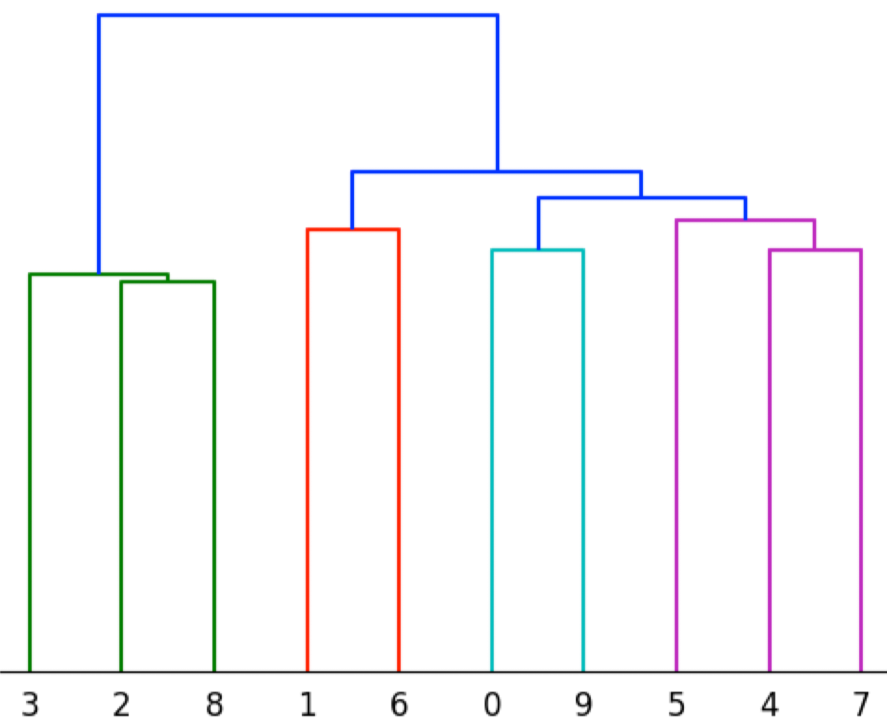
\includegraphics[width=.9\linewidth]{images/hierfig.png}
        %\caption{Hierarchical clustering of each class label in a 10-class example}
    \end{minipage}%
    \begin{minipage}[b]{.4\textwidth}
        \centering
        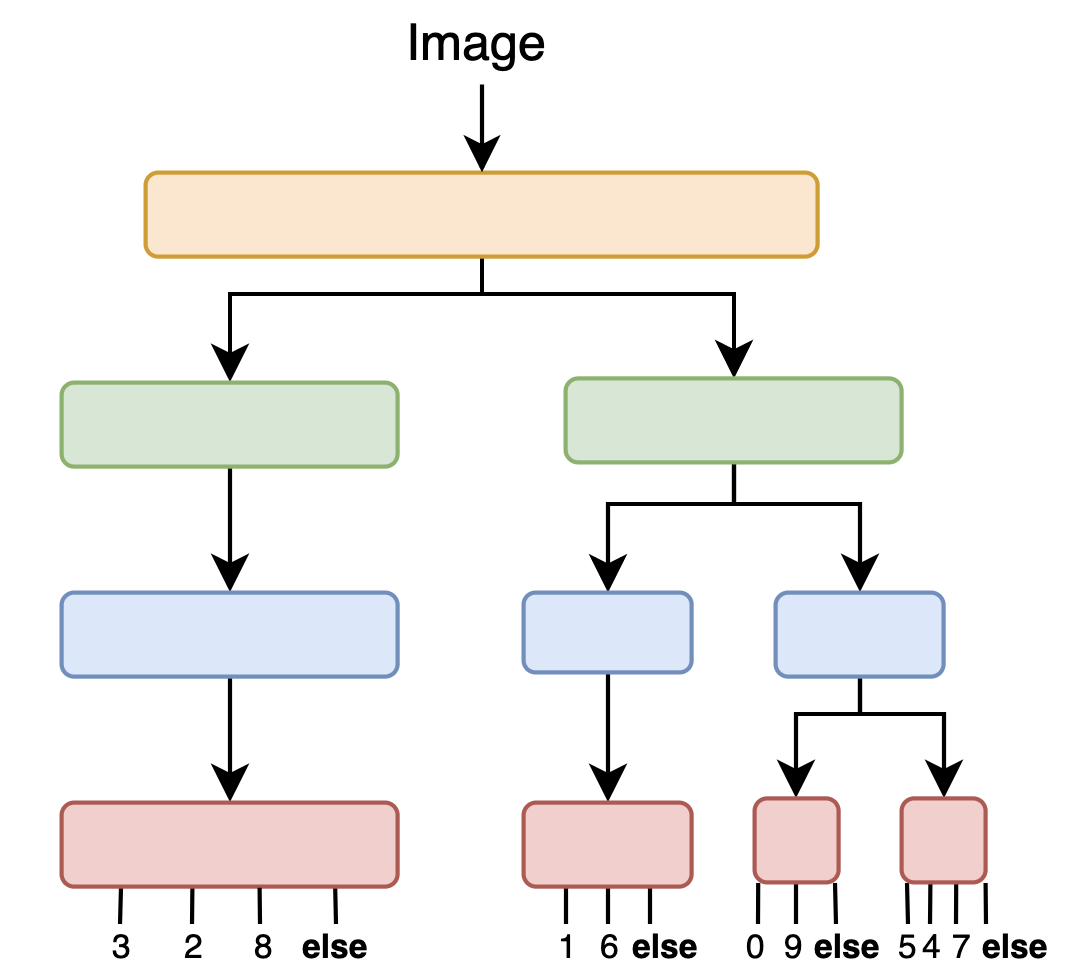
\includegraphics[width=.9\linewidth]{images/example_hier.png}
        %\caption{Hierarchical CNN obtained from the hierarchy on the left}
    \end{minipage}
    %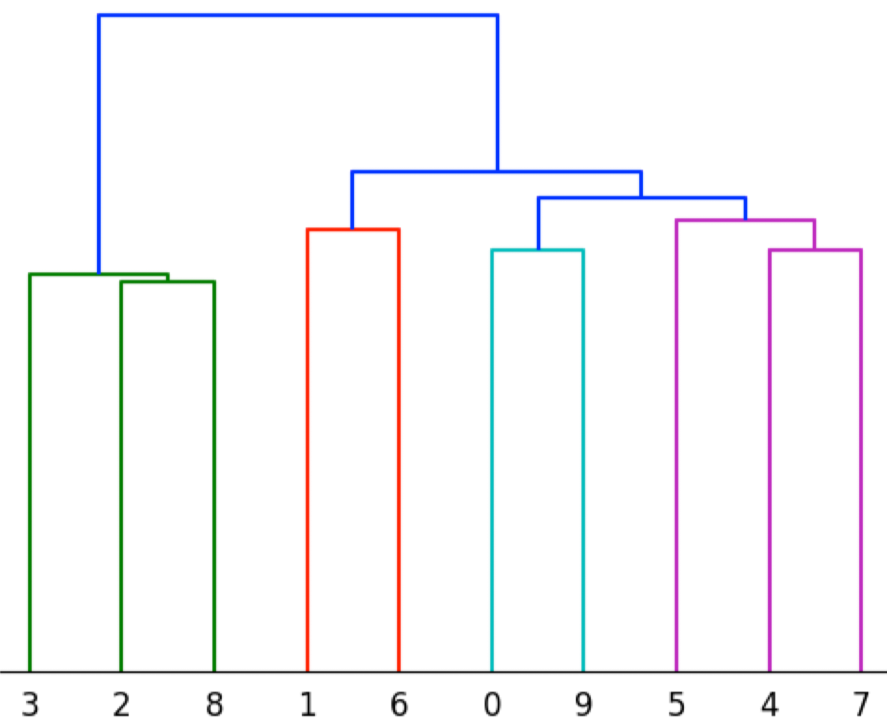
\includegraphics[width=0.40\textwidth]{images/hierfig.png}
    \caption{Hierarchical clustering of each class label in a 10-class example and the resulting network structure}
    \label{fig:hierarchy}
\end{figure}

\subsection{Hierarchy to CNN model}
\label{ssec:hiertoCNN}

Obtaining the hierarchy as described in \ref{ssec:hierarchy}, we construct our hierarchical CNN model. Depending on the hyper-parameters, such as depth of the tree, branching positions etc., there are many ways to construct the structure of hierarchical CNN with reference to the obtained hierarchy.

The structure is designed as a binary tree-shaped CNN, where the input image enters through the root layer.
Each layer takes the result of its parent layer as input and forwards its output to the next layer. 
Following the final output of the leaf layer is the classification layer for the subset of classes corresponding to that specific branch.
Note that, an extra classification label called 'else' is added to each leaves to detect classes that do not belong to a specific branch.
In the real-life scenario, if a user's model gives the output 'else', it means the encountered image has the class label that the user's model does not include.  
Therefore, additional model parts are downloaded until the image is recognized.

When constructing the tree-structured CNN, we followed some constraints as follows. 
In general, tree-structured CNN is designed by following a backbone network, such as VGG16 or MobileNet, as the base network, and branching it recursively to obtain a tree version of the network.
The structure is designed to be a binary tree, meaning a layer can only branch into two layers. 
Moreover, every path from the root to each leaf follows the same order of layers with the layer order of the backbone network.
Finally, the size of the resulting tree-structured CNN and the corresponding backbone network must be comparable. 
The reason is that if users end up using the entire tree-structured CNN, they would require only as much storage as the original backbone network.
To achieve this, after each and every branching, the number of convolutional channels in the following layers are reduced.

There are also hyper-parameters that affects the structure of the tree-based CNN. 
'Depth' hyper-parameter controls the number of times that the network can branch into two following networks. 
Moreover, 'branching positions' parameter controls where the branching happens.
For example, if the first position is '3', the network branches just after the 3rd convolutional layer in the backbone network.

In the light of all the above-mentioned constraints and hyper-parameters, the hierarchical CNN is constructed as in the figure \ref{fig:hierarchy}. 
In this simple example, the backbone network consists of four subsequent convolutional layer modules. 
'Depth' is set as 3 and 'branching positions are set as 1,2,3. 
Note that, reduced number of convolutional channels are represented as the size of the layers in the figure.
As an implementation rule, we do not split the branch if the remaining class labels in the branch is 3 or less. 
That is why the left branch in the figure is not divided into further sub-branches.

\section{Experiments}

\subsection{Generating user types and case study users}
\label{ssec:genusers}

Our method requires training users to create the hierarchy of our model as described in section\ref{ssec:hierarchy} and test users to test the final model in a scenario-based approach. 
We generated user data artificially in our work, therefore a realistic generation method is followed.
In our work, user data is defined as $\mathcal{D}_\mathrm{image} = \{\mathbf{I}_1,\mathbf{I}_2,\dots\}$, where each element represents an images a user encounters in their daily life. 
$\mathcal{D}_\mathrm{label} = \{c_1,c_2,\dots\}$ are the corresponding classification labels.
We can use as $\mathcal{D}_\mathrm{label}$ for obtaining the hierarchy as encountered labels are more important for training the hierarchy.

Our main assumption is that users interact with some classes significantly more than they interact with others due to their surroundings. 
Let us define the probability of users encountering class labels as $P=(p_1, \dots, p_C)$ where $\sum_{j=1}^C p_j = 1$ and $C$ is the number of different class labels.
To obtain these probabilities, we used Dirichlet distribution where the parameters of Dirichlet distribution are $(\alpha_1, \alpha_2, \dots, \alpha_C)$. 
The larger the $\alpha$ value is, the higher the probability output for the corresponding class label.
The output of the Dirichlet distribution determines each $P$.
We will refer to $P$ as user types for the rest of the paper.
All users will be generated according to one of the user type probabilities. 
User types can be interpreted as people with different surroundings, 
for example a chef is surrounded by kitchen tools whereas a pilot encounters airplanes on a daily basis.
Therefore, some probabilities are significantly higher than the others.

When choosing Dirichlet distribution parameters, we randomly put high values (200s) for more likely to encounter classes and low values (1s) for less likely to encounter classes. An example in 5-class classification would be $Dir(1,1,200,1,200)$. 
User type generated from this distribution will have high probability values corresponding to 3rd and 5th class labels.
A user generated from this user type will encounter images with class labels 3 and 5 much more than the rest of them. 

In our experiments with CIFAR-10, we randomly put 200s to 2 or 3 indices, which means users are likely to encounter 2 or 3 classes out of 10.
After creating the user types, users are generated, randomly following one of the user type probabilities $P$.
To generate a single user, a user type is chosen uniformly randomly between all user types. 
Then, set of encountered class labels for users, $\mathcal{D}_\mathrm{label} = \{c_1,c_2,\dots\}$, are generated according to the chosen user type. 
An example of list of encountered class labels would be, ${3,3,5,3,5,5,\dots,2,\dots,3,5,3}$ if generated from the distribution $Dir(1,1,200,1,200)$. 
It can be interpreted as the user usually encounters 3rd and 5th classes and sometimes encounters other classes as well.
Finally, random images from the dataset are collected corresponding to the class categories in the list to make scenario-based test users, $\mathcal{D}_\mathrm{image} = \{\mathbf{I}_1,\mathbf{I}_1,\dots\}$.

On a final note, training users are generated to construct the hierarchy of the system, whereas test users are generated to test our model as a scenario-based approach. 
Both training and testing users are from the same user types as we assume correlation between the requirements of all users. 

\begin{figure}
    \centering
    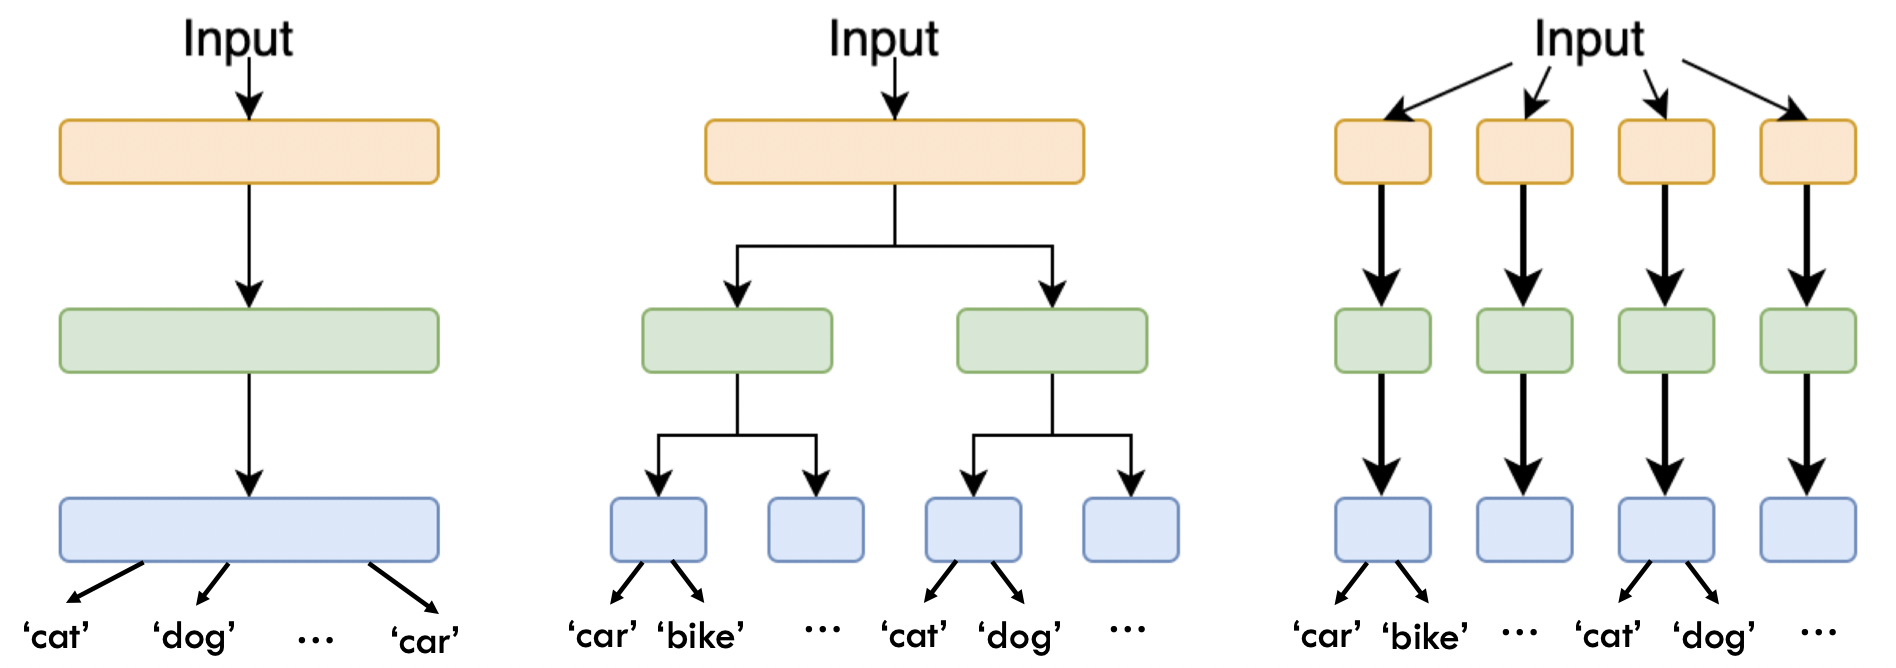
\includegraphics[width=0.9\textwidth]{thesis/images/classification_baselines-fig.png}
    \caption{Left is the regular CNN model. Middle one is the proposed hierarchical CNN. Right is the multiple smaller regular CNNs. Note that, all models are comparable in size.}
    \label{fig:baselines}
\end{figure}

\subsection{Baselines}
\label{ssec:baselines}
The whole network size of the hierarchical CNN and the baseline networks are approximately equal, because it would be fair to compare the networks with similar number of parameters. 
We constructed the hierarchical CNN simply by following a backbone network's layer order and splitting into sub-branches according to the obtained hierarchy. 

Another straightforward approach to our problem is using multiple backbone networks each reduced in size with the task of classifying a subset of classes. 
These subsets of classes corresponds to the same subsets of classes recognized in the leaf nodes of hierarchical CNN.
Same as the hierarchical CNN, we reduce the size of the each network to make the total sum of the number of parameters of all networks equal to the backbone network. 
We will refer to this method as multiple CNNs. 

In this method, none of the networks share parameters, thus decreasing the size of each network more than that of hierarchical CNNs by also reducing the number of parameters in the earlier layers. 
However, reducing the number of extracted low-level features from the input image in the early layers would result in a decrease of accuracy. 
The decrease in the accuracy is dire especially when the number of sub-networks is higher because we reduce the size of the each network more to balance with the backbone network size. 
We compare both the methods and the backbone network in terms of their accuracy and average memory consumption per user. 
All three architecture can be seen in the figure \ref{fig:baselines}.

\subsection{Dataset}

We evaluated our method on CIFAR-10~\cite{krizhevsky2009learning} dataset. 
CIFAR-10 is a relatively small dataset with 10 classes, consisting of 50000 training and 10000 test images with size 32 x 32 x 3.
The reason to choose CIFAR-10 is to try as many possibilities of constructing the hierarchy to find the best structure for the trade-off between accuracy and memory consumption.
Possible ways of constructing the Hierarchical CNN such as different depths, branching positions, etc., is tested on CIFAR-10 to find the ones with the best results with respect to both accuracy and memory cost. 
Then, in the future experiments, the best resulting models can also evaluated on bigger and more complex datasets.

\subsection{Backbone Networks}

As mentioned earlier in section \ref{ssec:baselines}, the hierarchical CNN and multiple CNNs are based on a backbone CNN, which means that they follow the convolutional layer order of another network.
In our work, VGG16~\cite{simonyan2014very} and MobileNet~\cite{howard2017mobilenets} are used as backbone networks.
Every branch starting from the root until the leaves follow the layer order of the backbone network. 
When the hierarchical CNN is split into two branches, although each branch still follows the layer order of the backbone network, the number of convolutional filters are reduced by a factor.
The reason is to maintain the overall size of the hierarchical CNN, therefore the storage consumption of the backbone network and the whole hierarchical CNN is the same which makes the comparison more fair.
Please note that, for CIFAR-10 experiments, we reduced the fully connected layer of VGG16 to prevent over-fitting, as VGG16 is designed to be used on larger domain classification problems.

\subsection{Implementation Details}

\subsubsection*{Training Phase}
Training users are generated as explained in \ref{ssec:genusers}. 
By examining the training users, the similarity between the classes can be calculated and the hierarchical clustering of class labels can be obtained, as in \ref{ssec:hierarchy}. 
Then, we construct the hierarchical CNN from the hierarchy.

When training the hierarchical CNN, every branch that leads up to a leaf node is trained with all the training images. 
Let's assume a simple example with two branches, meaning the backbone network is divided into two branches only once.
In this case, each image in the training dataset passes through the initial layers, then continues to pass the first branch and also the second branch subsequently.
Every leaf node consists of a subset of class labels and an extra label called 'else'. 
If a leaf node does not contain the class label of the training image, the branch is trained as though the label of the image is that special label 'else'. 
In our example, first the loss is calculated for the first branch and the initial layers and then the loss for the second branch and the initial layers is calculated. 
Note that, for the initial layers, loss from the first branch result and the second branch result is added to get the final loss. 
Loss calculation for more than 2 branches can be generalized in the same way.

To sum up, for each batch of training data, all branches starting from the root node and ending at a leaf node were trained together. Because some parameters between branches are shared, the shared parameters are updated according to the result of multiple leaf nodes.

\subsubsection*{Testing Phase}
In our experiments, two types of tests are conducted. 
First one is straightforward as we test the whole network of hierarchical CNN or multiple CNNs with the test set of CIFAR-10. 
The second type is the scenario-based testing, which imitates test users by using subsets of the test data.

As we emphasized throughout the paper, we assume that users encounter only a subset of all classes due to the limitation of their surroundings.
Therefore, we generated test users that are biased to encounter a subset of classes. 
The process of generating users and user types is explained in detail in section \ref{ssec:genusers}. 

For experiments on CIFAR-10, 10 user types are randomly generated and each user type is biased towards 2 or 3 random classes out of 10.
Then we generated test users that randomly belong to one of the user types. 
Each test user encounters a series of images that are biased to belong to some subset of all classes. 
Experiments are done with 100 generated test users for testing on CIFAR-10 where each test user encounters 1000 random images that are biased according to their user types.

In our scenario-based approach, users initially download the whole hierarchical model and use the whole model for the first $k$ classification task. 
This is the initial warm-up stage to learn the user's requirements.
Then, they only keep the part of the model including the formerly classified class labels and delete the rest of the model according to learned user requirements.
We will refer to the remaining part of the model as the personalized model.
In the future, if users encounter a class that is not part of the personalized model, the model detects that the newly encountered class belongs to another branch with the help of the 'else' classification label on every leaf in our tree-structured CNN (Figure \ref{fig:hierarchy}). 
As a result, they download additional parts of the model until the newly encountered class is recognized. 

The storage consumption per user is calculated as follows. 
Let us assume that a test user encounters 1000 images and personalized model was sufficient to recognize the class of the images $p$ times. 
The whole model is initially used $k$ times to learn the user requirements. 
$k$ is set to be 10 for our experiments.
The size of the whole model, personalized model and average size of the extra used model parts are $S_w$, $S_p$ and $S_{ex}$ respectively.
Then the calculation is done as the following.
\begin{equation}
    S_\mathrm{total} = [k(S_\mathrm{w}) + p(S_\mathrm{p}) + (1000-k-p)(S_\mathrm{p}+S_\mathrm{ex})] / 1000
\end{equation}
Finally, we take an average of $S_{total}$ over all the test users to obtain our final result for the storage consumption in our scenario.


\begin{table}
\begin{center}
\begin{tabular}{c||c|c|c||c|c|c}
\begin{tabular}[c]{@{}c@{}}Type of\\ Network\end{tabular} &
\begin{tabular}[c]{@{}c@{}}Number of \\ Parallel \\ Models\end{tabular} & 
Depth & 
\begin{tabular}[c]{@{}c@{}}Branching\\ Positions\end{tabular} & 
\begin{tabular}[c]{@{}c@{}}Test\\ Accuracy\end{tabular} & 
\begin{tabular}[c]{@{}c@{}}Scenario\\ Accuracy\end{tabular} & 
\begin{tabular}[c]{@{}c@{}}Number of\\ Params\\ (millions)\end{tabular}  \\
\hline\hline
VGG16& - & - & - & 89.33 & 88.38 & 15.25  \\ 
\hline
\hline
\multirow{3}{*}{\begin{tabular}[c]{@{}c@{}}Multiple\\ Smaller\\ CNNs\end{tabular}} 
& 2 & - & - & 88.54 & 88.57 & 9.9 \\ 
\cline{2-7} 
& 3 & - & - & 90.68 & 90.74 & 9.97 \\ 
\cline{2-7} 
& 5 & - & - & 89.89 & 89.78 & \textbf{7.89} \\ 
\hline
\hline
\multirow{10}{*}{\begin{tabular}[c]{@{}c@{}}Hierarchical\\ CNNs\end{tabular}} 
& - & 1 & 3 & 89.59 & 90.01 & 10.17 \\ 
\cline{2-7} 
& - & 1 & 6 & 91.08 & 90.89 & 10.33 \\ 
\cline{2-7} 
& - & 1 & 9 & 90.91 & 90.25 & 11.1 \\ 
\cline{2-7} 
& - & 2 & 3,6 & 90.69 & 90.64 & 9.52 \\ 
\cline{2-7} 
& - & 2 & 6,9 & 90.88 & 91 & 9.82 \\ 
\cline{2-7} 
& - & 2 & 3,9 & 90.58 & 90.64 & 9.72 \\ 
\cline{2-7} 
& - & 2 & 6,12 & 91 & 90.92 & 10.28 \\ 
\cline{2-7} 
& - & 2 & 9,12 & 90.79 & 90.41 & 11 \\ 
\cline{2-7} 
& - & 3 & 3,6,9 & \textbf{91.7} & \textbf{91.71} & \textbf{8.27} \\ 
\cline{2-7} 
& - & 3 & 6,9,12 & \textbf{91.75} & 91.54 & 9.11                                                                   
\end{tabular}
\end{center}
\caption[Comparison of Accuracy and Memory Cost on Image Classification task with VGG16]{\textbf{Comparison of Accuracy and Memory Cost on Image Classification task with VGG16}: Two methods are compared with the backbone network on the test accuracy, scenario accuracy and number of parameters.}
\label{ic-vgg16cifar10}
\end{table}


\subsection{Results}
As mentioned before, experiments are done on CIFAR-10. Results for the models using VGG16 as the backbone network can be seen in the Table \ref{ic-vgg16cifar10} where as results for MobileNet based models is in the Table \ref{ic-mobilenetcifar10}. 

The first three columns are the hyper-parameters. 
In this specific experiment, hierarchical CNN with depths 1, 2, 3 has 2, 3 and 5 leaf nodes or branches respectively due to the obtained hierarchy.
Also, they correspond to multiple CNNs with number of models 2, 3 and 5. 
Each corresponding model pairs have the same class labels on their leaf nodes.
Incidentally, note that depth is limited to 3 in CIFAR-10 experiments due to the number of classes.

Branching positions are generally chosen to be the convolutional layer positions that the number of kernels increase with respect to the previous layer in the backbone network. 
The reason is intuitive because otherwise the number of kernels would be less than the previous layer's as we reduce the number of kernels when branching. 
Having said that, it is also possible to choose all positions.

In both Table \ref{ic-vgg16cifar10} and \ref{ic-mobilenetcifar10}, best model overall is hierarchical CNN architecture with depth 3. 
Even though the number of parameters for multiple CNN with 5 models is the least, the accuracy drop is an issue because the number of parameters for first layers are less than that of hierarchical CNN.


\begin{table}
\begin{center}
\begin{tabular}{c||c|c|c||c|c|c}
\begin{tabular}[c]{@{}c@{}}Type of\\ Network\end{tabular} &
\begin{tabular}[c]{@{}c@{}}Number of \\ Parallel \\ Models\end{tabular} & 
Depth & 
\begin{tabular}[c]{@{}c@{}}Branching\\ Positions\end{tabular} & 
\begin{tabular}[c]{@{}c@{}}Test\\ Accuracy\end{tabular} & 
\begin{tabular}[c]{@{}c@{}}Scenario\\ Accuracy\end{tabular} & 
\begin{tabular}[c]{@{}c@{}}Number of\\ Params\\ (millions)\end{tabular}  \\
\hline\hline
MobileNet& - & - & - & 89.7 & 89.02 & 3.22  \\ 
\hline
\hline
\multirow{3}{*}{\begin{tabular}[c]{@{}c@{}}Multiple\\ Smaller\\ CNNs\end{tabular}} 
& 2 & - & - & 88.86 & 88.79 & 2.12 \\ 
\cline{2-7} 
& 3 & - & - & 88.37 & 88.43 & 2.16 \\ 
\cline{2-7} 
& 5 & - & - & 88.06 & 87.89 & \textbf{1.75}\\ 
\hline
\hline
\multirow{10}{*}{\begin{tabular}[c]{@{}c@{}}Hierarchical\\ CNNs\end{tabular}} 
& - & 1 & 3 & 89.64 & 89.46 & 2.13 \\ 
\cline{2-7} 
& - & 1 & 5 & 90.21 & 90.09 & 2.19 \\ 
\cline{2-7} 
& - & 1 & 8 & 90.09 & 89.71 & 2.45 \\ 
\cline{2-7} 
& - & 2 & 3,6 & 90.15 & 90.04 & 1.99 \\ 
\cline{2-7} 
& - & 2 & 5,8 & 90.16 & 89.84 & 2.08 \\ 
\cline{2-7} 
& - & 2 & 3,8 & 89.87 & \textbf{90.14} & 2.03 \\ 
\cline{2-7} 
& - & 2 & 5,11 & \textbf{90.6} & 90.11 & 2.18 \\ 
\cline{2-7} 
& - & 2 & 8,11 & 89.98 & 89.19 & 2.44 \\ 
\cline{2-7} 
& - & 3 & 3,6,9 & \textbf{90.27} & \textbf{90.12} & \textbf{1.82} \\ 
\cline{2-7} 
& - & 3 & 5,8,11 & 89.89 & 89.88 & 1.98                                                                   
\end{tabular}
\end{center}
\caption[Comparison of Accuracy and Memory Cost on Image Classification task with MobileNet]{\textbf{Comparison of Accuracy and Memory Cost on Image Classification task with MobileNet}: Two methods are compared with the backbone network on the test accuracy, scenario accuracy and number of parameters.}
\label{ic-mobilenetcifar10}
\end{table}




\lhead[\chaptername~\thechapter]{\rightmark}

\rhead[\leftmark]{}

\lfoot[\thepage]{}

\cfoot{}

\rfoot[]{\thepage}

\chapter{Faster ANN}
\label{FasterANN}

\section{Method}

\begin{figure}
    \centering
    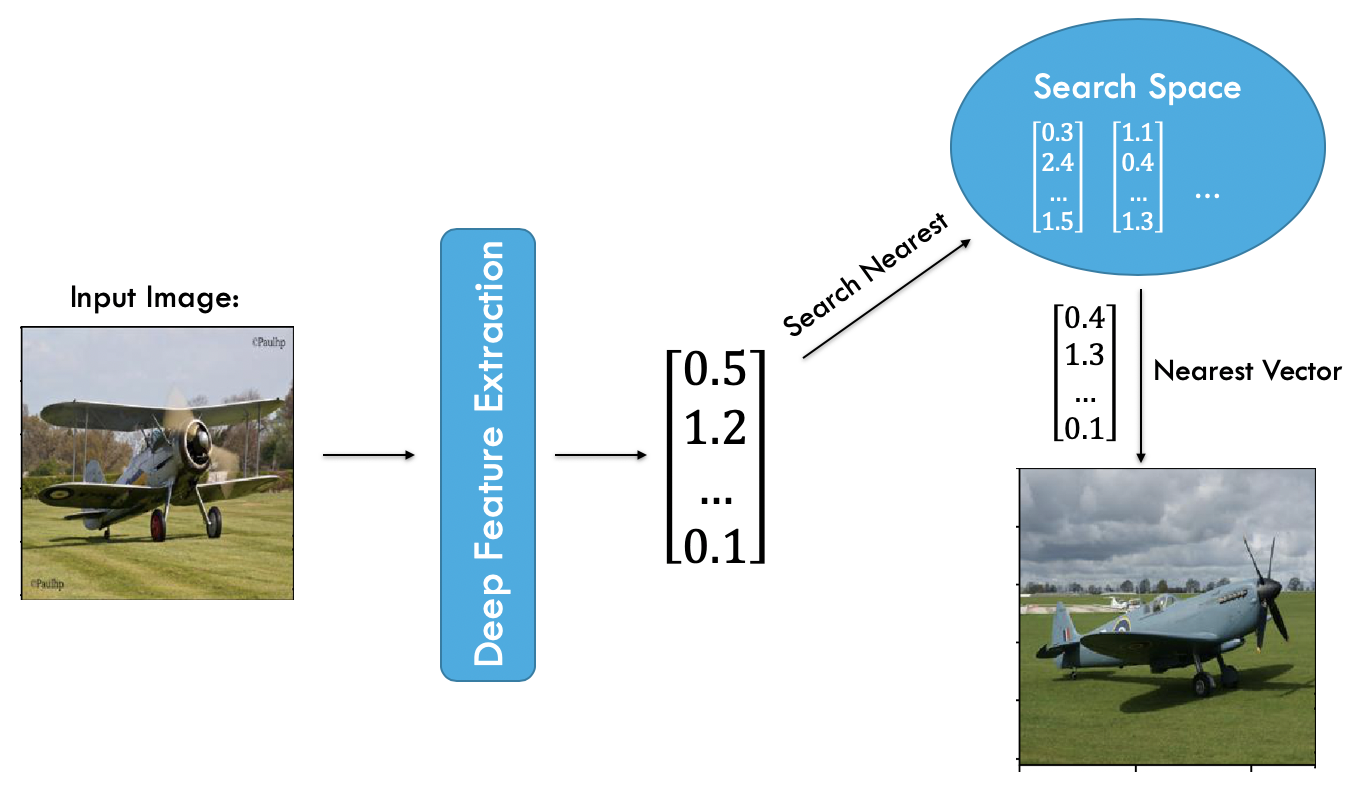
\includegraphics[width=0.9\textwidth]{thesis/images/image_ret_exp-fig.png}
    \caption{Overview of Image Retrieval}
    \label{fig:ret-exp}
\end{figure}

In image retrieval task, images are represented as vectors and the aim is to search a database of vectors for the nearest vector to the input image, as in figure \ref{fig:ret-exp}. 
For each query vector $\mathcal{Q} = \{\bm{q}_1,\bm{q}_2,\dots\} \subset \mathbb{R}^D$ and database vectors $\mathcal{X} = \{\bm{x}_1, \dots, \bm{x}_N\} \subset \mathbb{R}^D$, the task is to retrieve the most similar image with $n^* = \underset{n\in\{{1,\dots,N}\}}{\mathrm{argmin}} \vert\vert \bm{q} - \bm{x_n} \vert\vert $ for each query vector. 

Naive approach would be brute-force searching the entire database.
However, exhaustive searching of the database is slow and costly, especially with vectors with large dimensions. 
Thus, Approximate Nearest Neighbor (ANN) search algorithms are proposed with significantly faster search speed and a small probability of error. 
We built our work on the FAISS implementation~\cite{faiss} of Product Quantization~\cite{jegou2010product} with inverted multi-index as well as using it as our baseline.

As explained in section \ref{subsec:related-quantization}, product quantization method clusters the database space into $K$ clusters using k-means algorithm, $\mathcal{X}_1,\dots,\mathcal{X}_K$ where $\bigcup_{i=1}^K \mathcal{X}_i = \mathcal{X}$ and $\mathcal{X}_i \bigcap \mathcal{X}_j = \emptyset$. 
We will refer to these clusters as subspaces or cells.
Then, the database vectors are assigned into one of $\mathcal{X}_k$.
When a query vector $\bm{q}\in\mathbb{R}^D$ is searched, first the nearest $\mathcal{X}_k$ is retrieved. 
Then, all vectors $\bm{x}\in\mathcal{X}_k$ is traversed to find the nearest vector.

Our work aims to reduce the area of the search space by limiting the number of comparisons in the first step with $\mathcal{X}_k$ for each user according to their requirements. 
ANN search algorithms commonly assume that the distribution of the query vectors is the same with the distribution of the database vectors. 
However, real users have diverse query distributions, different than that of the database, 
so they query some parts of the search space more and the other parts less likely. 
This difference is sourcing from their limited surroundings in daily life or their different hobbies and interests. 
By utilizing this idea, we can reduce the search space by limiting the comparisons only to the relevant $\mathcal{X}_k$ for each user according to their requirements.

\begin{figure}
    \centering
    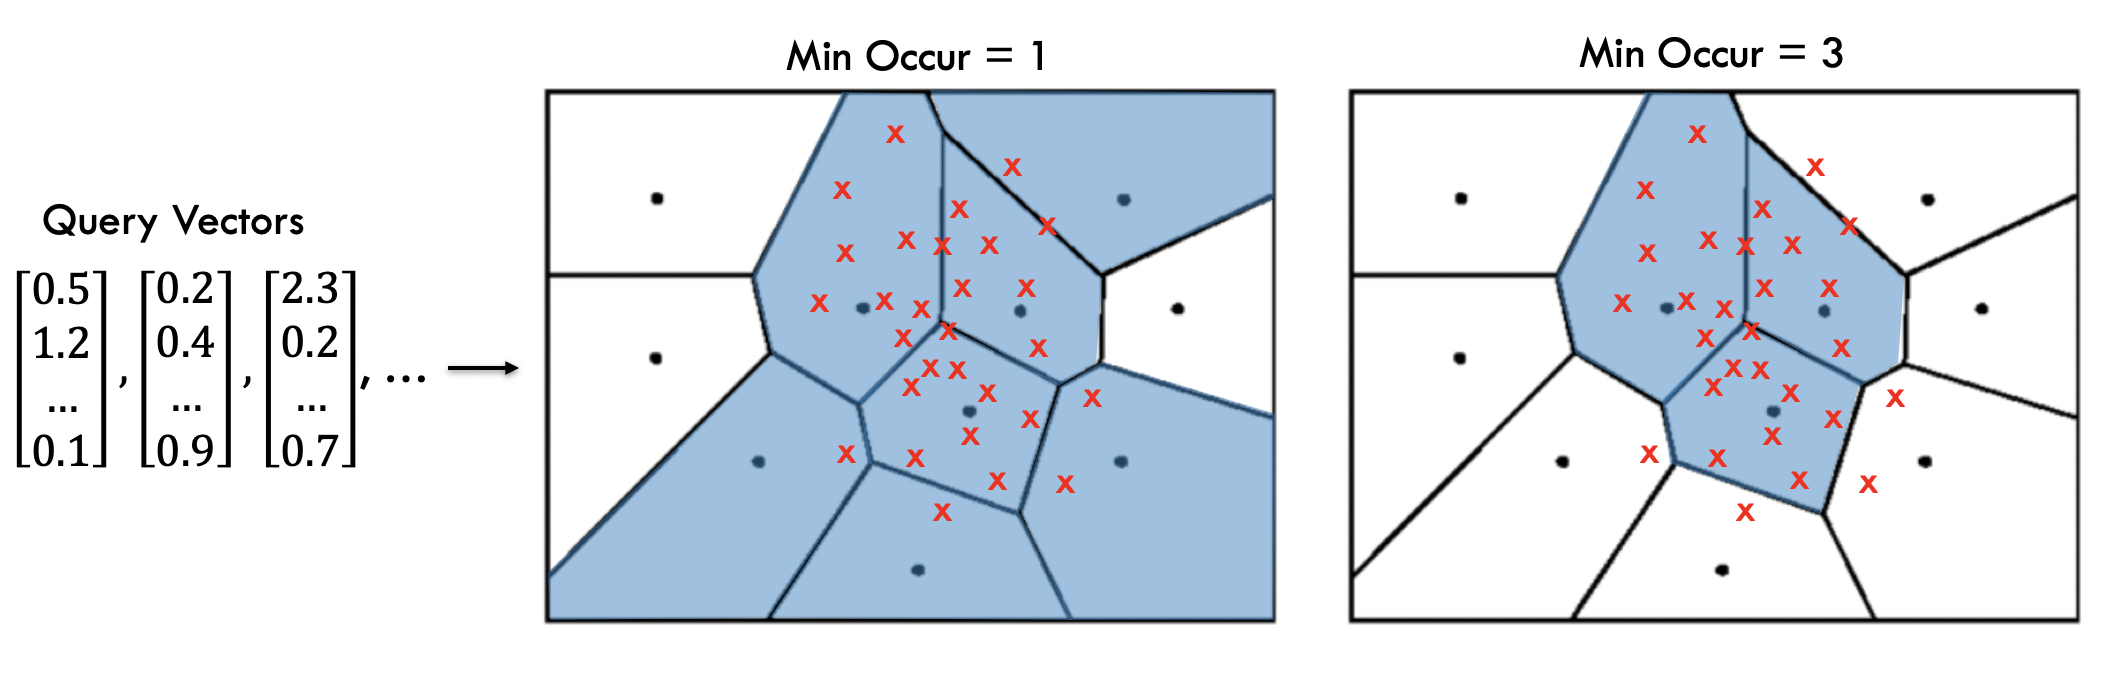
\includegraphics[width=\textwidth]{thesis/images/improvement-fig.png}
    \caption{Query vectors and clustering of the search space is shown. Red crosses represent the position the query vectors fall in the space. We can choose to include every subspace with red crosses in our search as in the left figure. A hyper-parameter can control to include a subspace according to minimum occurrence of red crosses.}
    \label{fig:motivation}
\end{figure}

In figure \ref{fig:motivation}, query image examples of a user is shown with red crosses on the search space. 
For this user, a new query vector just needs to be compared with centroids in blue areas. 
We can reduce the amount of centroids to compare with a simple hyper-parameter, controlling whether to include a subspace according to minimum occurrence of the past query vectors. 
In this way, we can adjust the trade-off between accuracy and the speed of the system.

In the following subsections, our work will be explained in detail. 
Firstly, the details of using classification label information to reduce the area of search space will be explained. 
Next, the dataset and the distribution of class labels to subspaces will be discussed.
Then, the method of representing the images with vectors will be described in detail. 
After specifying the implementation details, baselines of our work will be defined.

\subsection{Using classification label information}

In our method, we used classification labels to represent the user requirements. 
Given the classification labels $\mathcal{C} = \{1,2,\dots,C\}$ where $C$ is the number different of labels, each user requirement is defined as $\mathcal{U} \subseteq \mathcal{C}$. 
Assuming we know the classification labels of our database vectors, $\mathcal{X}$ can be redefined as $\mathcal{X} = \{(\bm{x_1}, c_1), \dots, (\bm{x_N}, c_N)\}$.
Then, the subspaces will also contain the class labels, $(\bm{x}, c) \in \mathcal{X}_k$.

Given a user requirement $\mathcal{U}$ to our system, we choose the corresponding subset of all subspaces according to the following algorithm.
If any of $(\bm{x}, c) \in \mathcal{X}_k$ contains the class label $c \in \mathcal{U}$, we consider that subspace as a relevant subspace to our user.
Let us define the relevant subspaces as $\mathcal{X}_\mathrm{rel} \subseteq \{\mathcal{X}_1,\dots,\mathcal{X}_K\}$.

In the search part of our algorithm, the query vector $\bm{q} \in \mathbb{R}^D$ is compared with the representative vectors of $\mathcal{X}_\mathrm{rel}$ instead of all the $\{\mathcal{X}_1,\dots,\mathcal{X}_K\}$. 
The remaining part of our algorithm is the same with the original PQ method.
Once the nearest $\mathcal{X}_k$ is found, the vectors associated with that subspace are traversed to find the nearest vector.

Our method accelerates the coarse quantization part of the PQ algorithm, where finding the closest subspace is the objective. 
We show the significance of accelerating the first part of PQ as the following.
Following the convention, we chose $K=\sqrt{N}$ where $N$ is the number of database vectors. 
In this way, number of vectors corresponding to $\mathcal{X}_k$ will be $\sqrt{N}$ in average. 
Once a query vector comes, the algorithm searches the closest centroid among $\sqrt{N}$ centroids. 
Then, the query vector is compared with the database vectors that belong to the chosen $\mathcal{X}_k$ and a few neighboring ones. 
In both steps, there are $O(\sqrt{N})$ comparisons to be done. 
Therefore, accelerating the first part is as important as accelerating the second part.

\subsection{Dataset and Distribution of Class Labels to Subspaces}
\label{retrievallabelinfo}

In our experiments, we used the scene recognition dataset called Places365~\cite{zhou2017places}. 
There are 1.8 million training images with 365 class categories. 
1.3 million out of all images is used to construct our search database. The remaining images are used to train the ANN algorithm and also for the query vectors.
The class categories include various scenes such as airport terminal, library, train station, waterfall, etc. 
With such diverse scenes, users would interact with only a subset of the class categories and our idea can be easily applied to speed up the search according to each user's requirements.

\begin{figure}
    \centering
    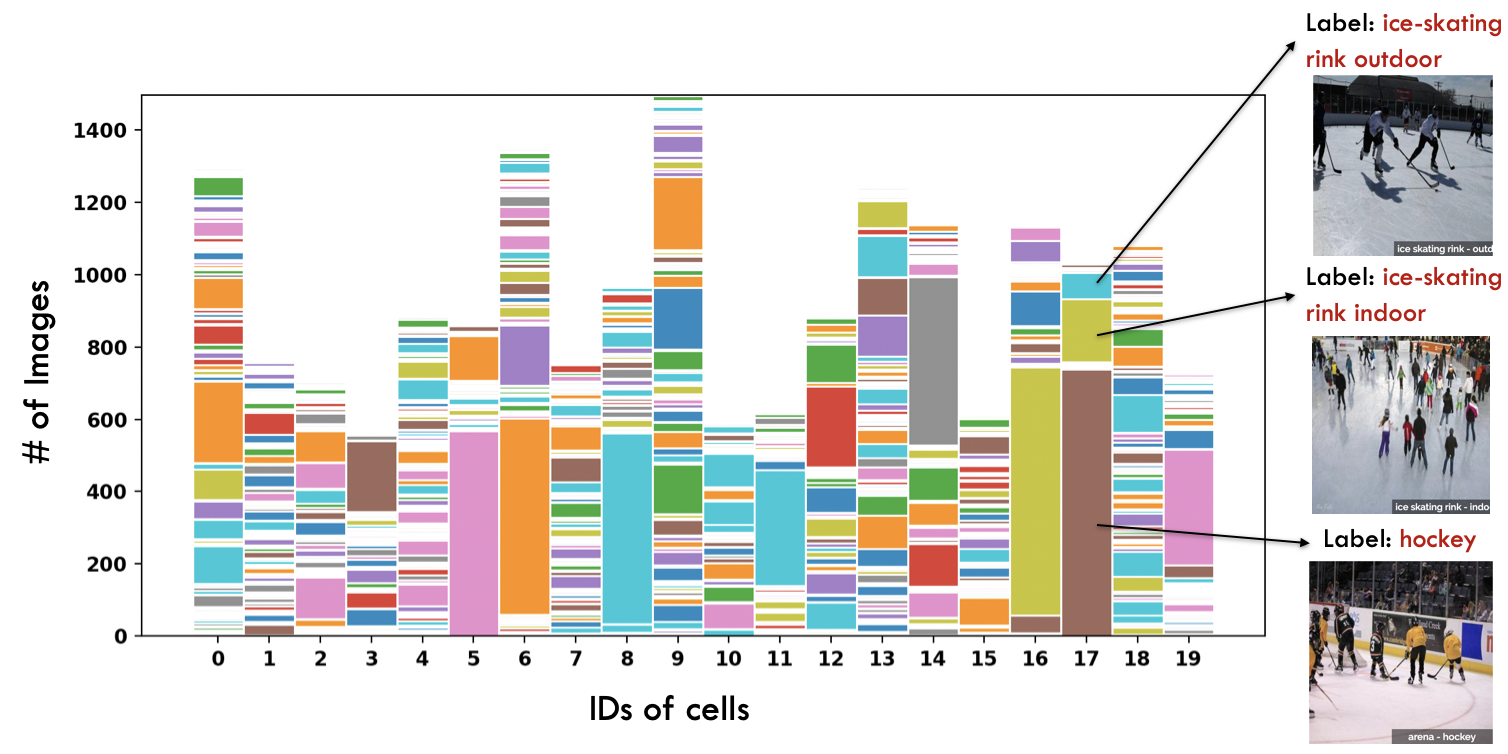
\includegraphics[width=\textwidth]{thesis/images/label_dist-fig.png}
    \caption{Distribution of the images according to their class labels in the first 20 subspaces}
    \label{fig:label-dist}
\end{figure}

Following the convention, we chose the number of subspaces as $K=\sqrt{N}$ where $N$ is the number of database vectors. 
Therefore, the search space is divided into 1140 subspaces which is the square root of the number of images($\sqrt{N}$) in our search database. 
Distribution of the images to those subspaces according to their classification labels can be seen in the figure \ref{fig:label-dist}.
As can be seen in the figure, some subspaces have extreme bias towards a few class, while others do not have much. 
There are many class categories in Places dataset that have similar images, such as "elevator-door", "elevator-interior", "elevator lobby", "elevator shaft", etc.
For example, the subspace with id:17 in the figure has labels with very similar images.


\subsection{Extracting Deep Features of Images}
\label{extractdeepfeatures}

\begin{figure}
    \centering
    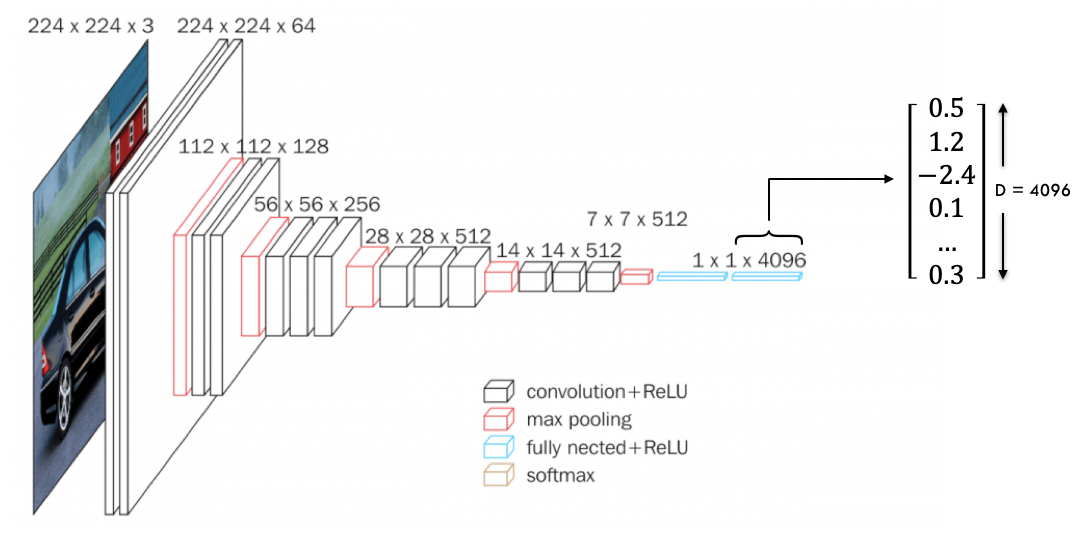
\includegraphics[width=0.9\textwidth]{thesis/images/deep_features-fig.png}
    \caption{Last fully connected layer of VGG16~\cite{simonyan2014very} is discarded to obtain a descriptor vector with dimension 4096.}
    \label{fig:vec-repr}
\end{figure}

In the work of Babenko \emph{et al.}~\cite{babenko2014neural}, using a pre-trained convolutional neural network in ImageNet for image retrieval task is shown to have decent results. 
Note that, it is also shown that if the network is trained on the same data with the retrieval dataset, the results are better.
However, instead of getting the best performance, we simply investigate the comparison of our idea with the current best methods.
Therefore, we used VGG16~\cite{simonyan2014very} network that is pre-trained on ImageNet~\cite{deng2009imagenet}. 
The last fully connected layer is discarded to get a vector representation with 4096 dimensions, as in figure \ref{fig:vec-repr}.
Then, all database images are passed through the model once to get their descriptor vectors.

However, dimensions of the vectors were quite big for both storage and calculation. 
As stated in \cite{jegou2012negative}, applying whitening on the descriptor vectors not only helps with the computational and storage costs, but also improves the accuracy of retrieval tasks.
We applied Principal Component Analysis (PCA) to obtain the final descriptor vectors with 64 dimensions.


\section{Experiments}

\subsection{Implementation Details}

As mentioned before, we built our work on FAISS implementation~\cite{faiss} of product quantization with inverted index, namely IndexIVFPQ. 
The code is shared publicly and we modified the code to tailor to our needs.
Extra function is added to adjust the search space according to a given list. 
This function is called during the indexing phase of the database before the search.

The training phase is required for IndexIVFPQ and it needs different vectors than the database vectors with similar distribution.
Training dataset of Places365 contains 1.8 million images. 
After obtaining the descriptor vectors of the images, we split the vectors into three parts.
Base vectors containing roughly 1.3 million vectors to form the search space, about a half million training vectors to train IndexIVFPQ and remaining approximately 3000 for query vectors.
The vectors are split into 3 parts in a way that the number of images for each label in all parts are almost equal.
When querying for a user, only the images with the required labels out of 3000 are used for the query images.

\subsection{Baselines}

Our main baseline is the FAISS implementation~\cite{faiss} of product quantization with inverted index, namely IndexIVFPQ.
We compared our method with IndexIVFPQ by evaluating both method for search time per query and recall at 1 where recall at $k$ checks if the true result is one of the $k$ predicted results. 

\subsection{Experiments}

\begin{figure}
    \centering
    \begin{minipage}[b]{.5\textwidth}
        \centering
        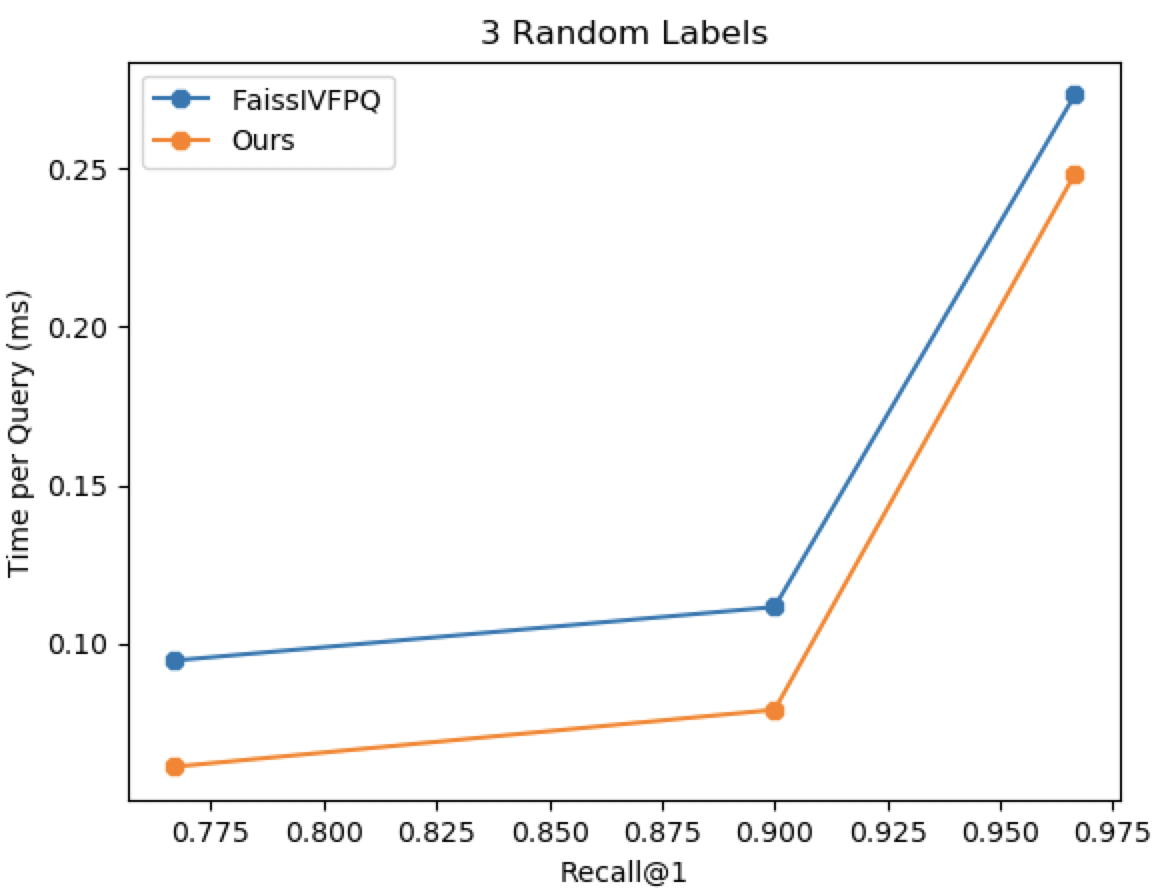
\includegraphics[width=.9\linewidth]{thesis/images/3_random.png}
        % \caption{Results for 3 random label}
        \label{fig:randomexpsub1}
    \end{minipage}%
    \begin{minipage}[b]{.5\textwidth}
        \centering
        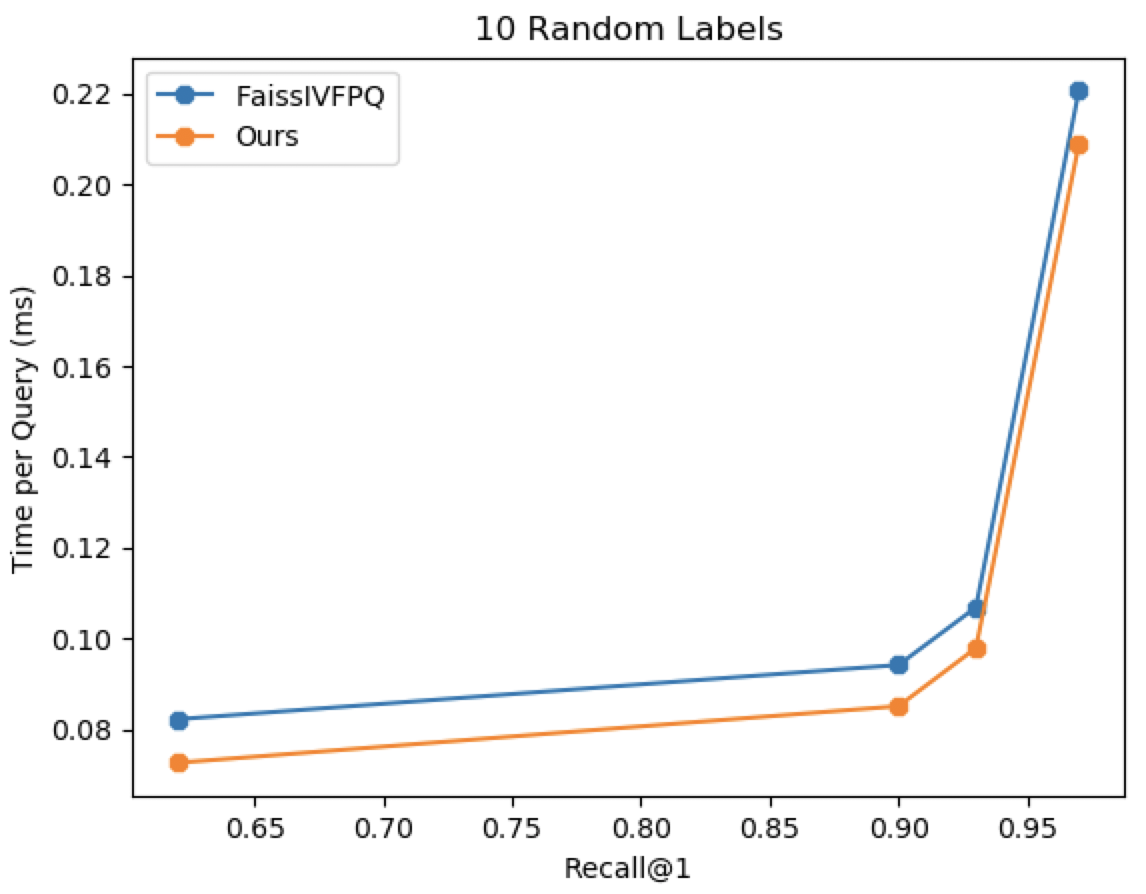
\includegraphics[width=.9\linewidth]{thesis/images/10_random_only_mo1.png}
        % \caption{Results for 10 random label}
        \label{fig:randomexpsub2}
    \end{minipage}
    %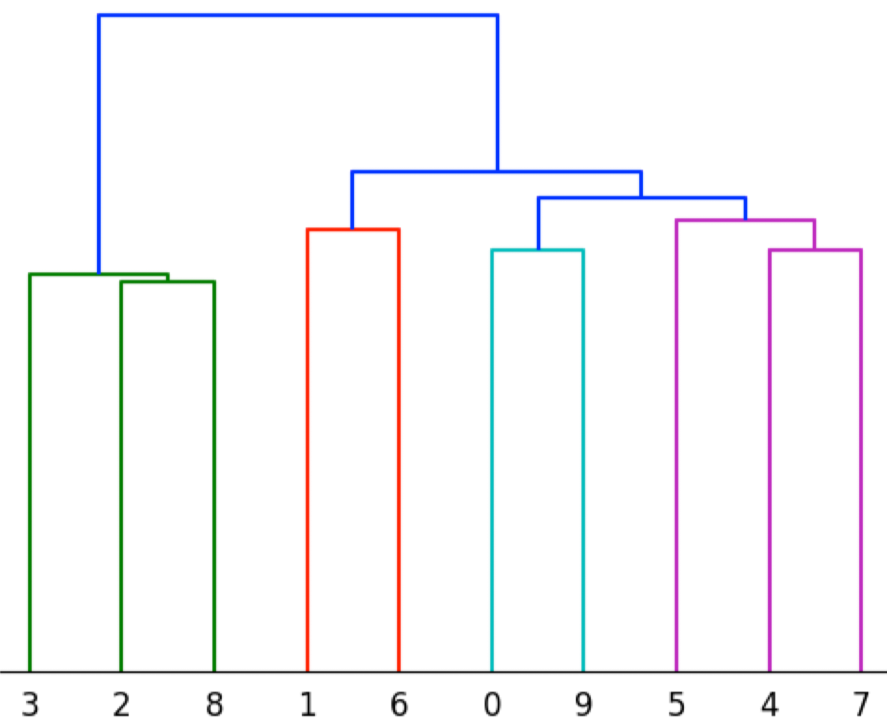
\includegraphics[width=0.40\textwidth]{images/hierfig.png}
    \caption{Comparison of our method with FaissIVFPQ on randomly picked labels as user requirements}
    \label{fig:randomexp}
\end{figure}

According to our scenario, users have wearable devices with a camera, such as wearable glasses or a smart phone. 
When they first start using the image search system, the class recognition system will store the classification labels of the users. 
After storing labels for enough time, we will consider those labels as the user's required class labels.
Then, we select the subspaces, out of all 1140 subspaces, that contain any of those class labels at least $m$ times. 
$m$ is the hyper-parameter to adjust the trade-off between accuracy and speed.
Whenever a new query image comes from the user, we compare the query vector only with the centroids of the selected subspaces to reduce time.
Note that, classification labels are merely a tool for us to categorize the requirements of the users.
Most similar images do not necessarily have the same labels.

In our experiments, two types of tests are conducted. 
The first phase of testing is done with random or hand-picked data to analyze our method thoroughly. 
For the second phase of testing, real data is used to observe whether our method is applicable to real-life scenarios. 
Two phases will be explained in their respective sections.

\subsubsection*{Experiments with Artificial Data}

\begin{figure}
    \centering
    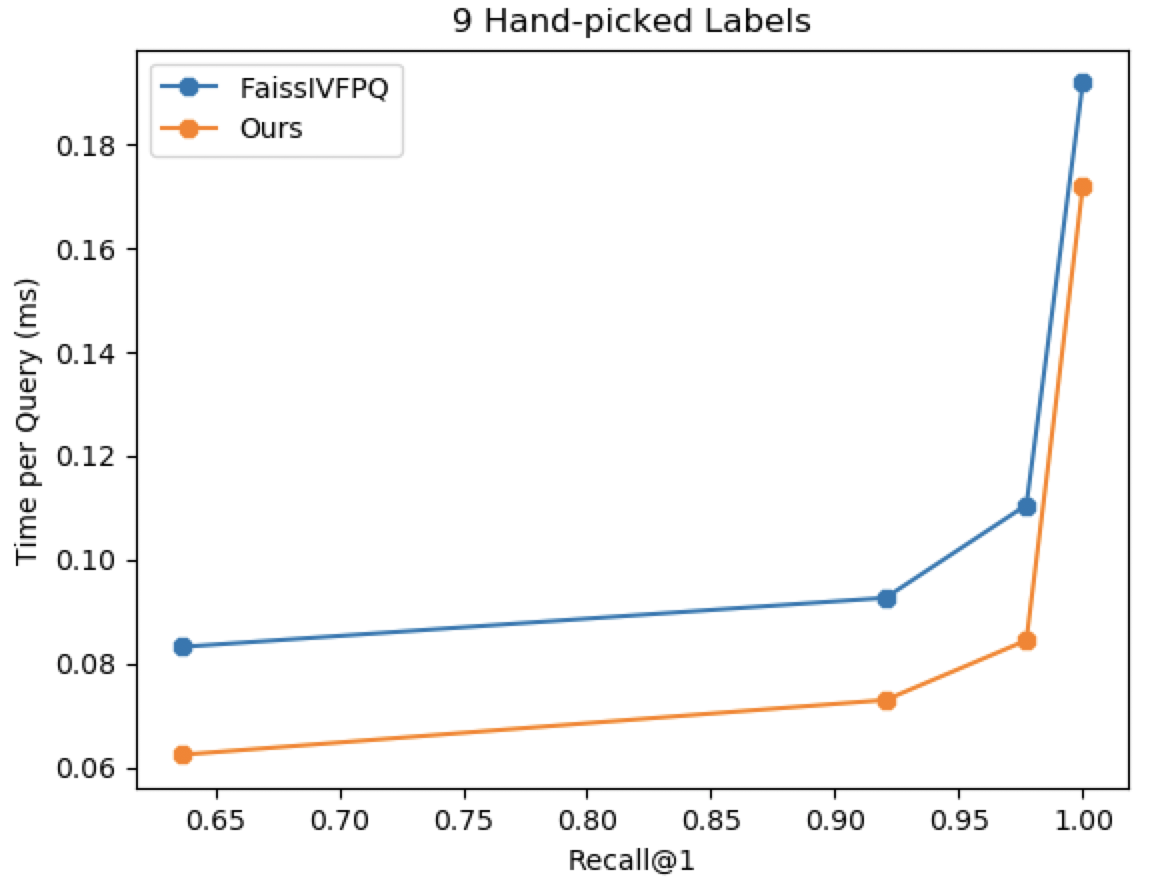
\includegraphics[width=0.8\textwidth]{thesis/images/9_handpicked.png}
    \caption{Comparison of our method with FaissIVFPQ on hand-picked labels as user requirements}
    \label{fig:handpickedexp}
\end{figure}

Our proposed method is making use of the user requirements to speed up the search for image retrieval. 
In our work, user requirements are represented with the classification labels. 
These are the labels that the users most likely encounter in their daily lives. 
According to our scenario, these labels are extracted with a recognition model included in their device as mentioned earlier in \ref{retrievallabelinfo}. 
In our experiments, we either randomly picked or hand-picked these labels to validate our method with diversified tests.

When the class labels are randomly picked, the results are expected to be the worst for our method. 
The reason is that randomly picked labels would not be related to each other, whereas in real life user-required labels might have similar images. 
Because the task is similarity search, similar images with different labels are closer in the search space, therefore it is easier to reduce the space more.
For example, randomly picked labels might include labels such as volcano, waterfall, ski slope at the same time, whereas user-required labels are more likely to have labels such as campus, library-outdoor, library-indoor.
Having said that, results for randomly picked labels can be seen in the figure \ref{fig:randomexp}.
In both of the figures, it can be clearly seen that our method surpasses the baseline as our method can perform faster with the same accuracy.

Further experiments are done with hand-picked labels. 
In these experiments, labels are picked intuitively considering their relevancy. 
The results can be seen in the figure \ref{fig:handpickedexp}. 
We can see again that our method performs better than the baseline.
Note that points in the graphs are taken by changing the nprobe parameter. 
After finding the closest subspace to the query vector, the algorithm searches for a few neighboring ones. 
The number of subspaces to check is controlled with nprobe.


When the number of labels chosen for user requirements is relatively small, our method outperforms the baseline method.
However, as the number of labels go up, our method starts to behave similarly to the baseline.
The reason is that we only search the sub-spaces in our search space which contains at least $k$ of any required labels. 
When the number of labels is high, it becomes harder to exclude some sub-spaces. Because almost all of them has at least one of any required labels. 
That is why, our method works if user required labels are relatively small which actually makes sense because if the user requires many labels, they do not need to use our system as they can use generic model for their need.


\subsubsection*{Experiments with Real Data}

\begin{figure}
    \centering
    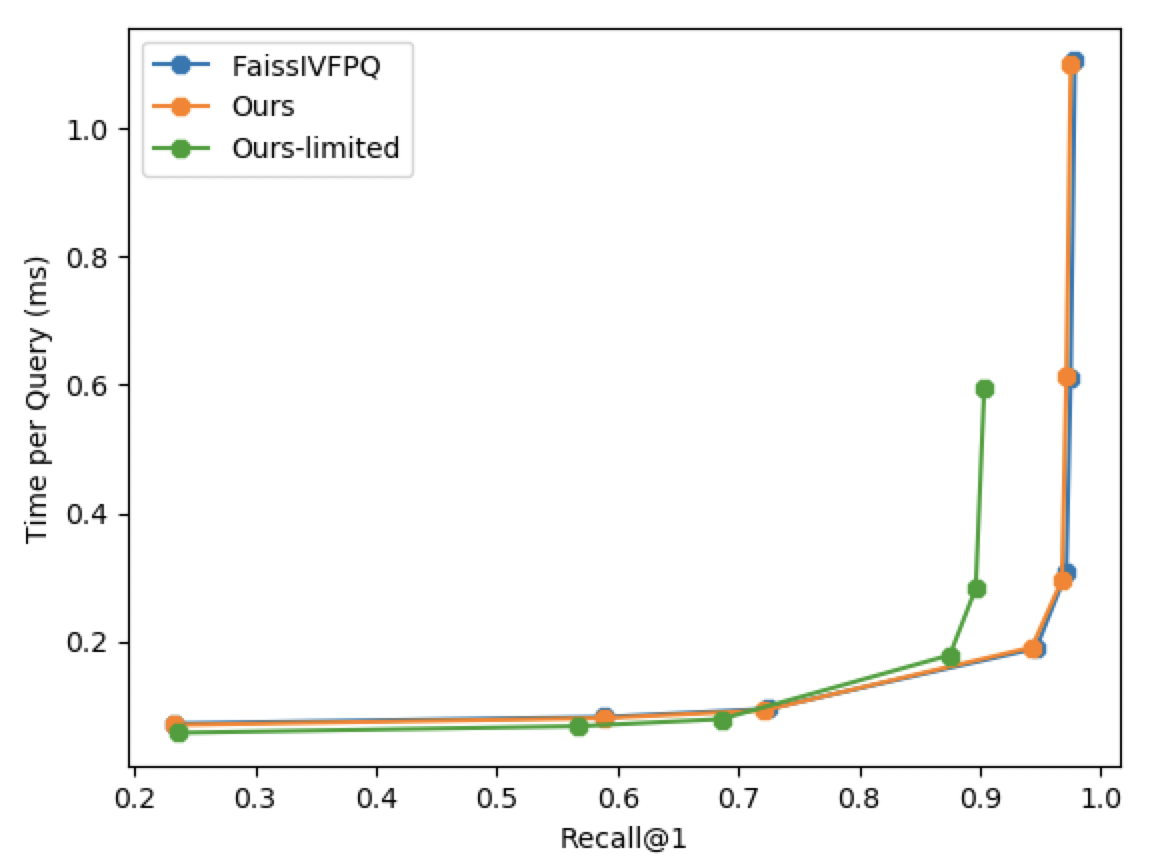
\includegraphics[width=0.8\textwidth]{thesis/images/real_data_experiment.png}
    \caption{Comparison of our method with FaissIVFPQ in a real-life experiment}
    \label{fig:realdataexp}
\end{figure}

The real data for this phase is obtained using GoPro Hero8 with a chest mount. 
Daily v-logs are taken for 2 days, first day data is used for extracting user required classification labels and second day data is used to actually test our method.

Daily v-logs are recorded for 2 days for nearly a total of 2 hours. 
Videos are mostly taken when the subject is on the move to prevent recording constant same scenes.
For each day, videos are sampled with a ratio of 1 frame per 10 seconds. 
426 frames for the first day and 280 frames for the second day is obtained.

First day frames are classified with a pre-trained ResNet with 18 layers~\cite{resnet}. 
73 different labels are recognized from 426 frames with many misclassified labels such as airplane cabin, airport terminal, berth, catacomb and many more. 
Many labels are predicted only once or with little probabilities. Therefore, a limit is put to probability and minimum occurrence to exclude some of the labels. 
We refer to this method as "Ours-limited".

Second day frames(280) are converted to query vectors with the usual process, explained in \ref{extractdeepfeatures}. The result of searching with these query images is shown in the figure \ref{fig:realdataexp}. 
There are 1140 sub-spaces in the search space. Our method could reduces the area to only 1108 sub-spaces using 73 user-required labels. 
Thus, our method fails to speed up the baseline for the real-life experiment. 
Limited version of our method is obtained by a limit to probability by 50 percent classification accuracy and at least 3 minimum occurrence of labels to count them as requirements.
However, excluding some classified labels reduced the accuracy of "Ours-limited".
Results will be discussed more thoroughly in the next chapter and further experiment results will be shown in \ref{Appen} Additional Results.



\lhead[\chaptername~\thechapter]{\rightmark}

\rhead[\leftmark]{}

\lfoot[\thepage]{}

\cfoot{}

\rfoot[]{\thepage}

\chapter{Discussion}
\label{discussion}

\section*{Image Classification}

The evaluation of our work is done on CIFAR-10 dataset using VGG16 and MobileNet models. 
Using both models for the backbone of the hierarchical CNN, our method successfully reduced the size of the model for each user while maintaining the accuracy. 
Moreover, it can be seen that the accuracy of our method is slightly higher than the backbone networks.
The backbone networks are originally designed to classify larger classification problems with many training data. 
The reason could originate from our training method, however we used the same training scheme for all the models. 
Splitting the network into branches to obtain hierarchical network actually reduces the size of the network for each branch and make classification in each branch more suited to the task at hand, as smaller size models are more suitable with CIFAR-10 classification task.
Having said that, we believe that our hierarchical CNN could produce relatively less accuracy when it is a bigger classification task such as ImageNet. 
Accuracy is not the only concerning issue when it comes to training our model for a larger classification task. 
Another concern is that obtaining the best hierarchy would be really challenging. Further discussion about our future work will be done in the next chapter.

According to our results, both the accuracy and the memory consumption become better as the depth increases. However, further experiments should be conducted with a bigger dataset. 
Multiple smaller CNNs also showed good results as the memory consumption decreases significantly with a little drop in accuracy. 
However, the little drop in the accuracy could be significantly larger when the experiments are done on a larger dataset.

All our experiments are conducted with artificial user preferences. Even though we followed a realistic scheme, further experiments with real users are required. 

\section*{Image Retrieval}

Experiments are done with both artificial data and real-life data. 
The results with the artificial data clearly showed that our method can successfully increase the search speed by making use of user requirements.
However, the results of the experiments with the real-life data was not as good as we expected. 

There are several reasons to explain the bad performance with the real-life data. 
Sampling images from the videos is done automatically by extracting an image in every 10 seconds. 
These sampled images are both used in training phase to obtain user requirements as classification labels and in testing phase as query vectors.
However, quality of some images are bad. They are either too dark or blurred to understand. Some bad image examples can be seen in the figure \ref{fig:baddata}.

Our method depends heavily on the classification of training images to learn user requirements. 
Not only the classification accuracy is important, but also the number of classified labels has a direct effect on the search space reduction and consequently on the speed up rate.
However, pre-trained models achieve around 50\% Top-1 accuracy for the classification task on Places365 dataset.
We used pre-trained ResNet-18 architecture in our experiments and many of our training data is classified incorrectly (Figure \ref{fig:wrongly}).
Because of this, even in 426 training images, 73(out of 365) different class labels are predicted. 
While this number is too large for nearly a 1-hour video, we confirmed that there are many unrelated classification labels.

Large number of classified labels led us to limit the number of classification labels by the classification accuracy and the number of occurrences.
Unfortunately, the accuracy of our method is affected considerably.
There is a huge correlation between correctly classifying an image and correctly converting an image to its vector representation.
In our experiments, pre-trained VGG16 is used to obtain descriptor vectors from the images.
Therefore, there is a big possibility that the vectors are not representing the database images accurately.

Having said all of the above, our method is shown to perform well in ideal settings. 
Even in the worst settings, the performance of our method is similar to the baseline method. 


\begin{figure}
    \centering
    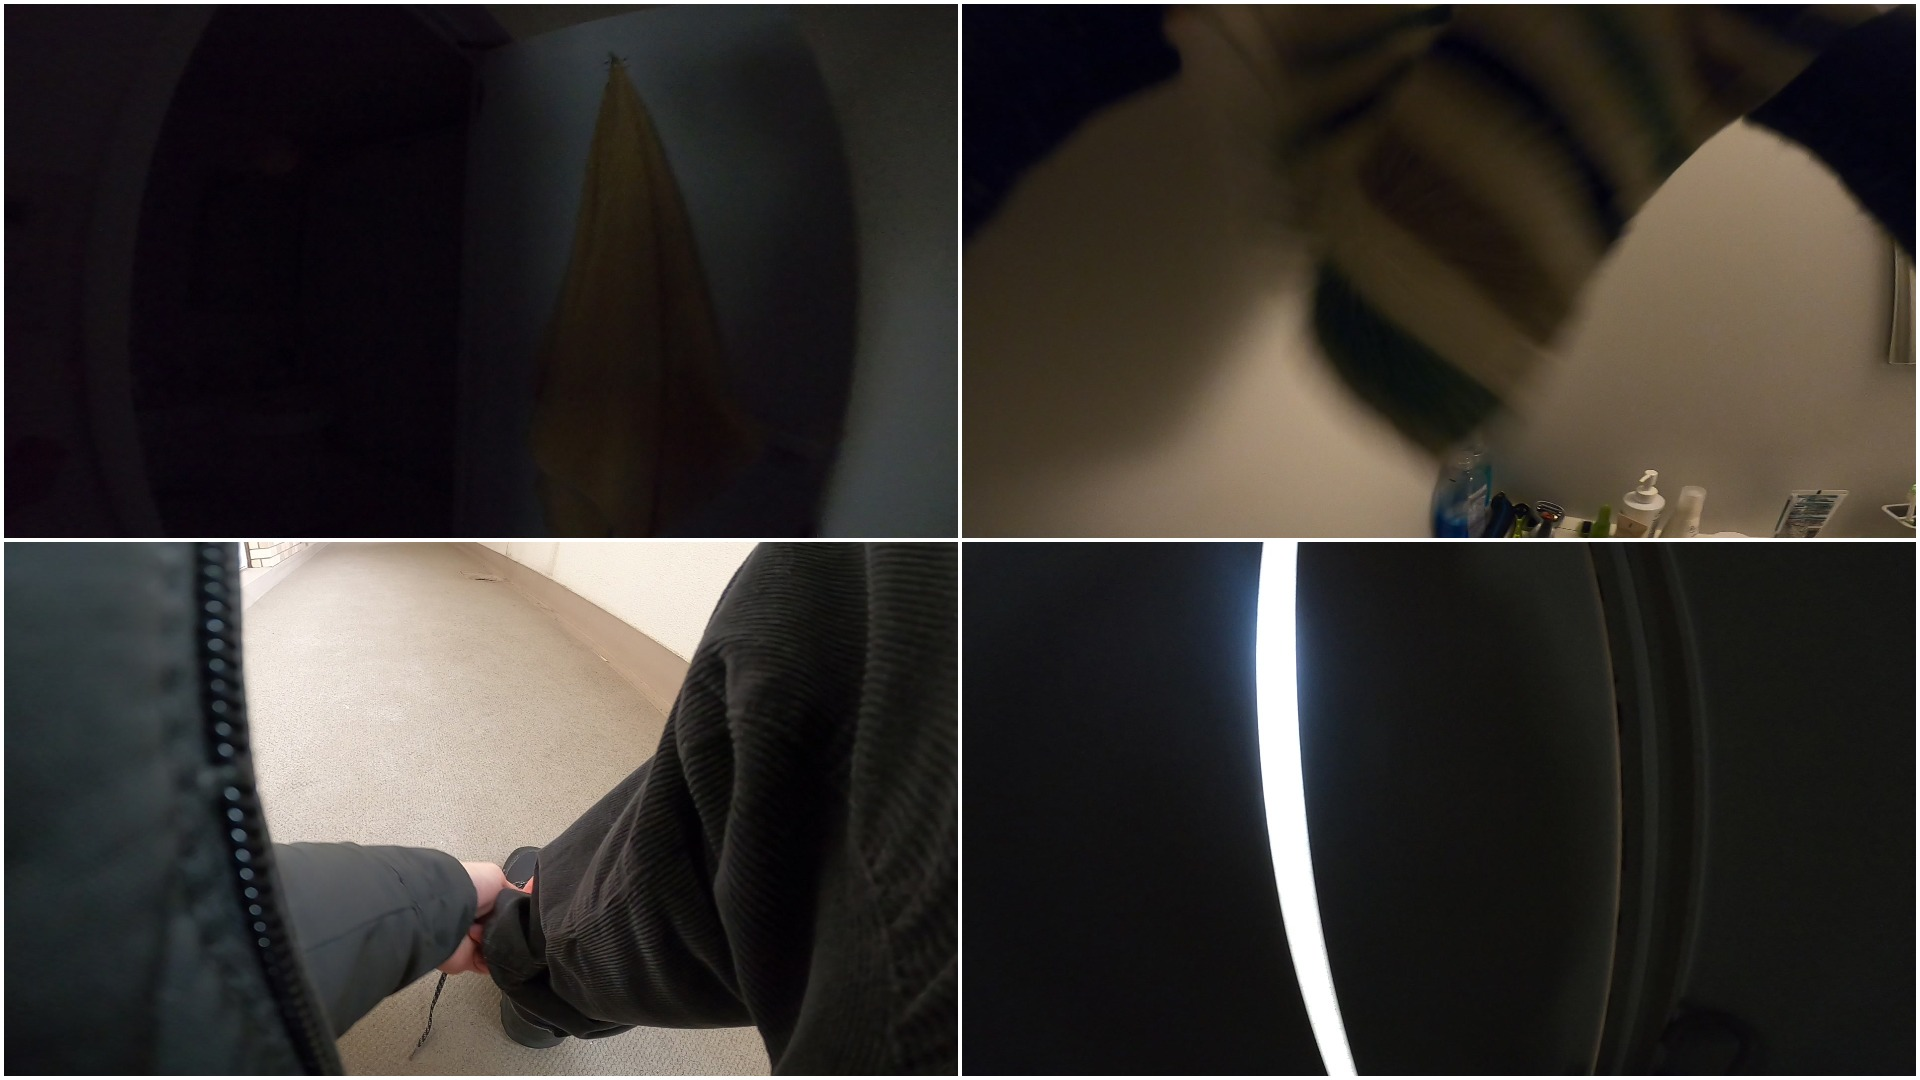
\includegraphics[width=0.8\textwidth]{thesis/images/ret-bad-images.jpg}
    \caption{Bad image examples in the test data.}
    \label{fig:baddata}
\end{figure}

\begin{figure}[ht] 
  \begin{subfigure}[b]{0.5\linewidth}
    \centering
    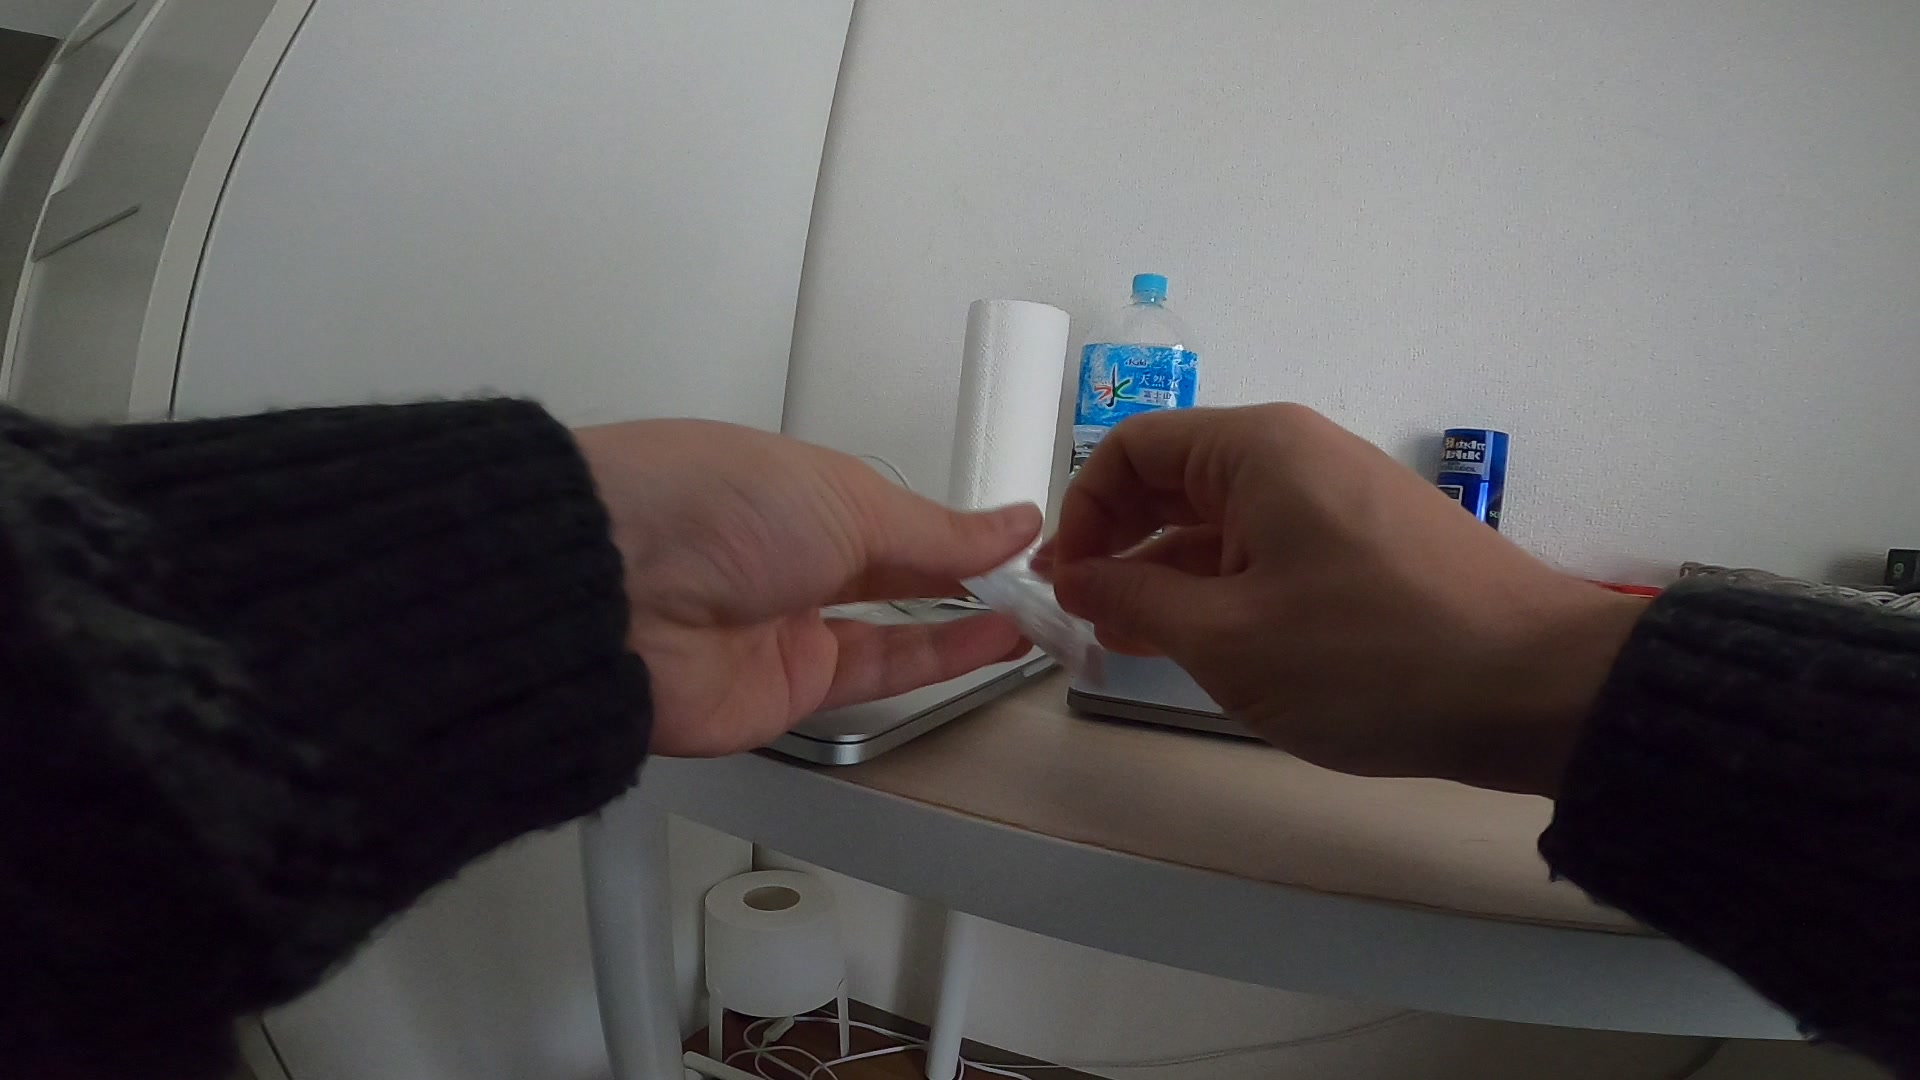
\includegraphics[width=0.75\linewidth]{{thesis/images/temp/1_beautysalon(0.63)}.jpg} 
    \caption*{Beauty Salon (63\%)}
    \vspace{4ex}
  \end{subfigure}%% 
  \begin{subfigure}[b]{0.5\linewidth}
    \centering
    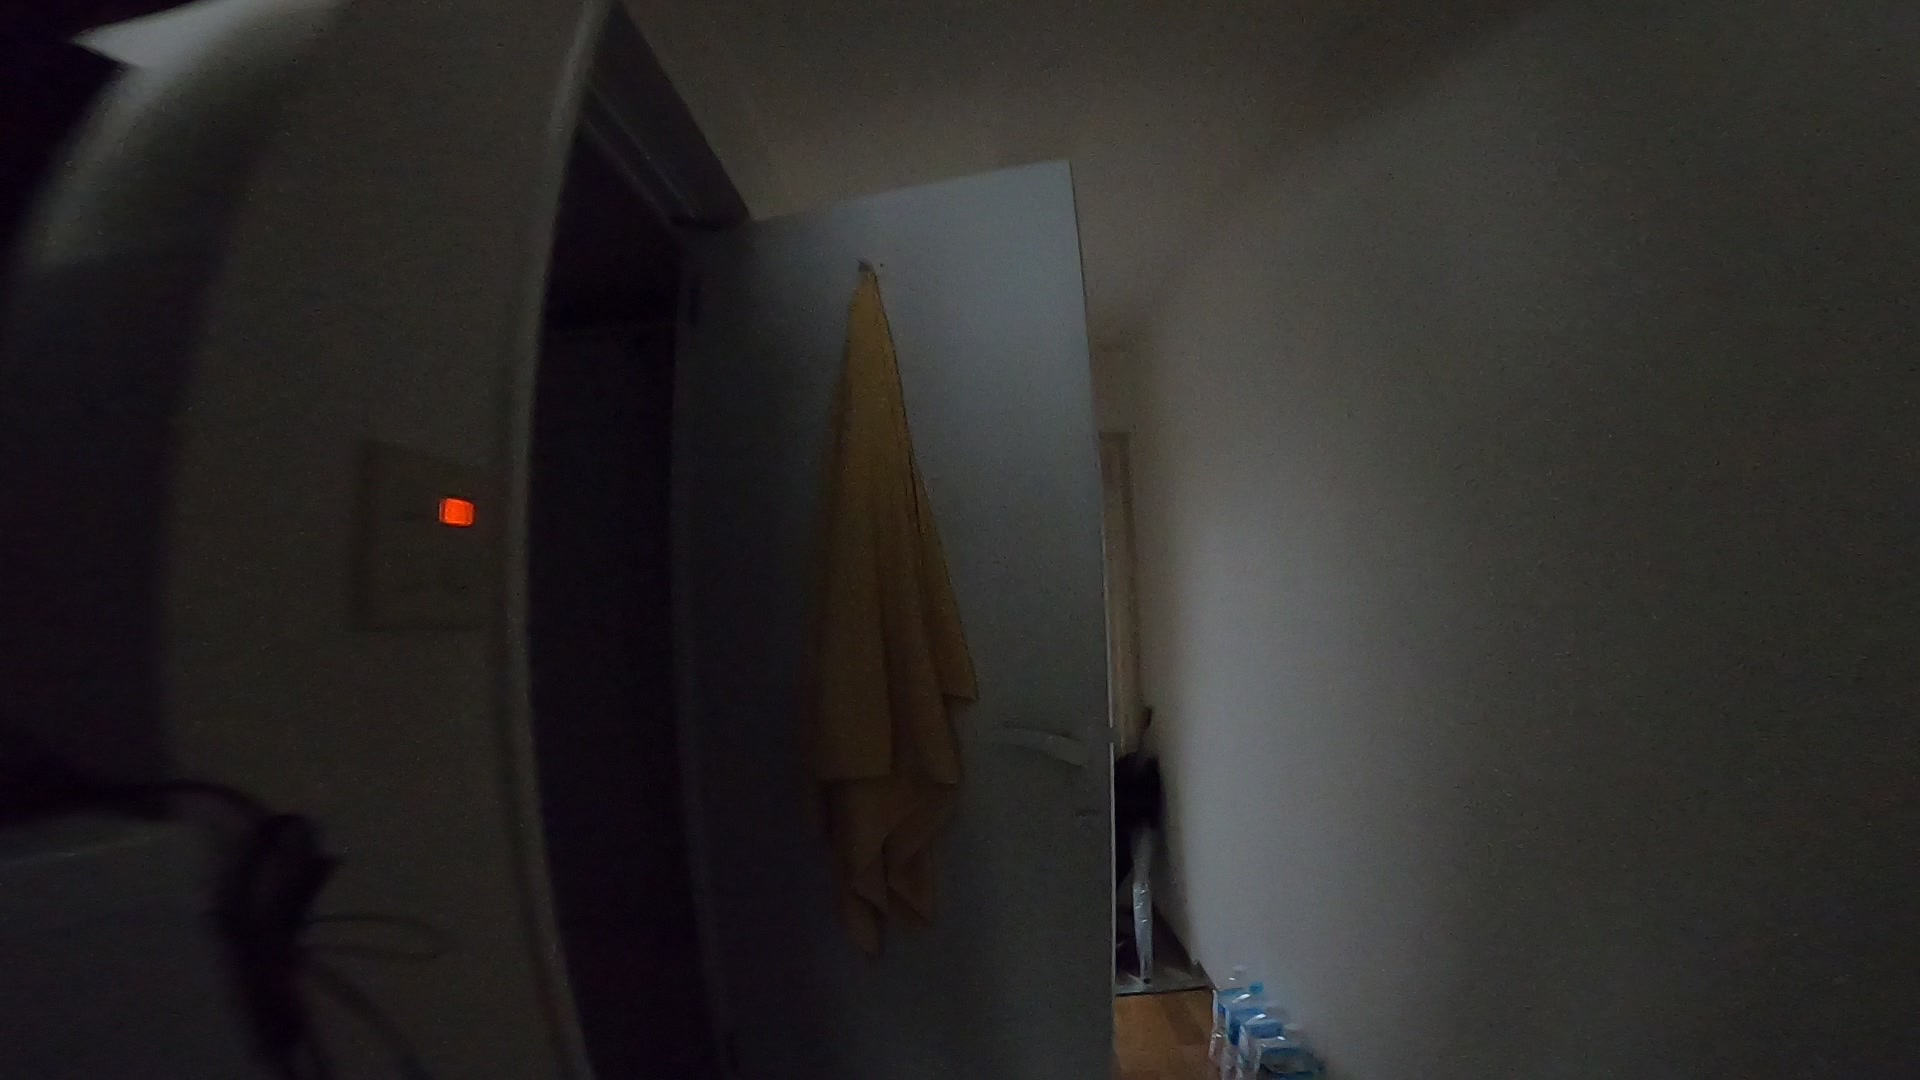
\includegraphics[width=0.75\linewidth]{{thesis/images/temp/3-alcove(0.11)}.jpg} 
    \caption*{Alcove (11\%)} 
    \vspace{4ex}
  \end{subfigure} 
  \begin{subfigure}[b]{0.5\linewidth}
    \centering
    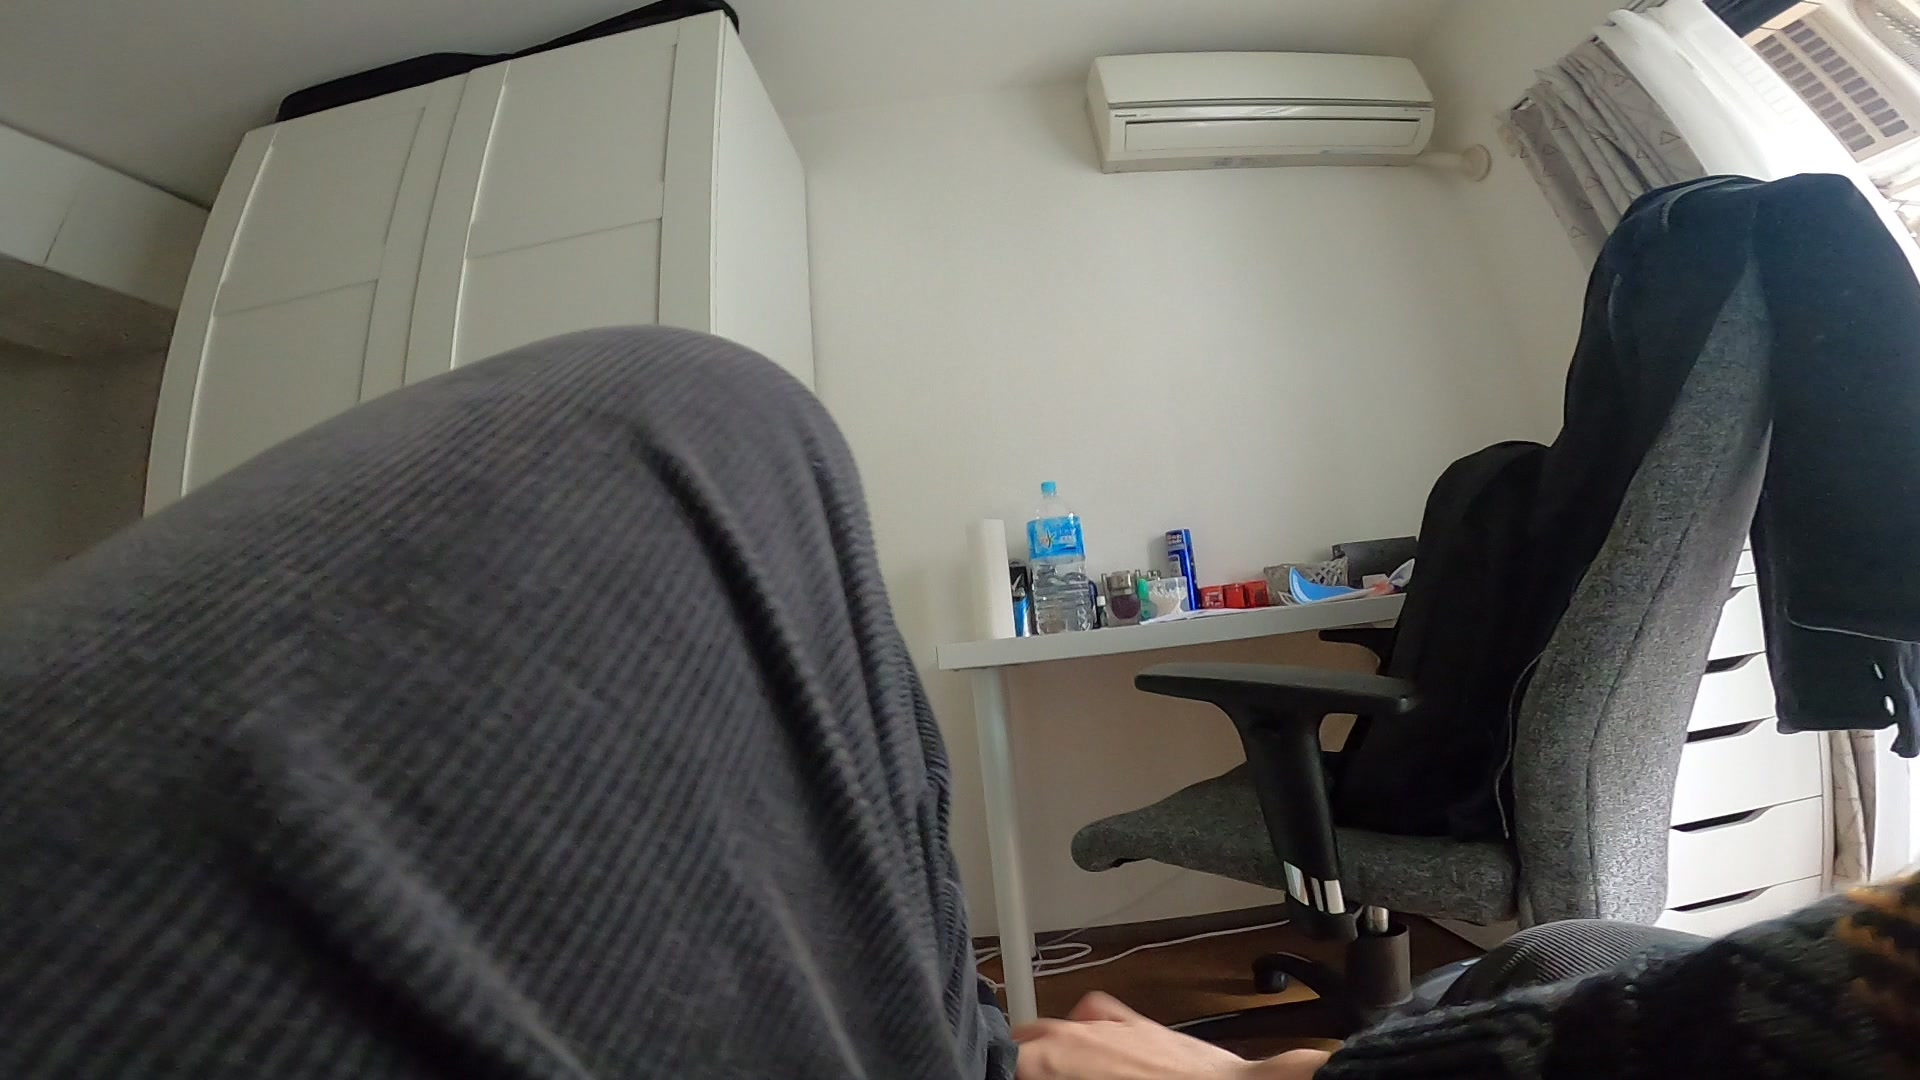
\includegraphics[width=0.75\linewidth]{{thesis/images/temp/4-airplanecabin(0.70)}.jpg} 
    \caption*{Airplane Cabin (70\%)} 
    \vspace{4ex}
  \end{subfigure}%%
  \begin{subfigure}[b]{0.5\linewidth}
    \centering
    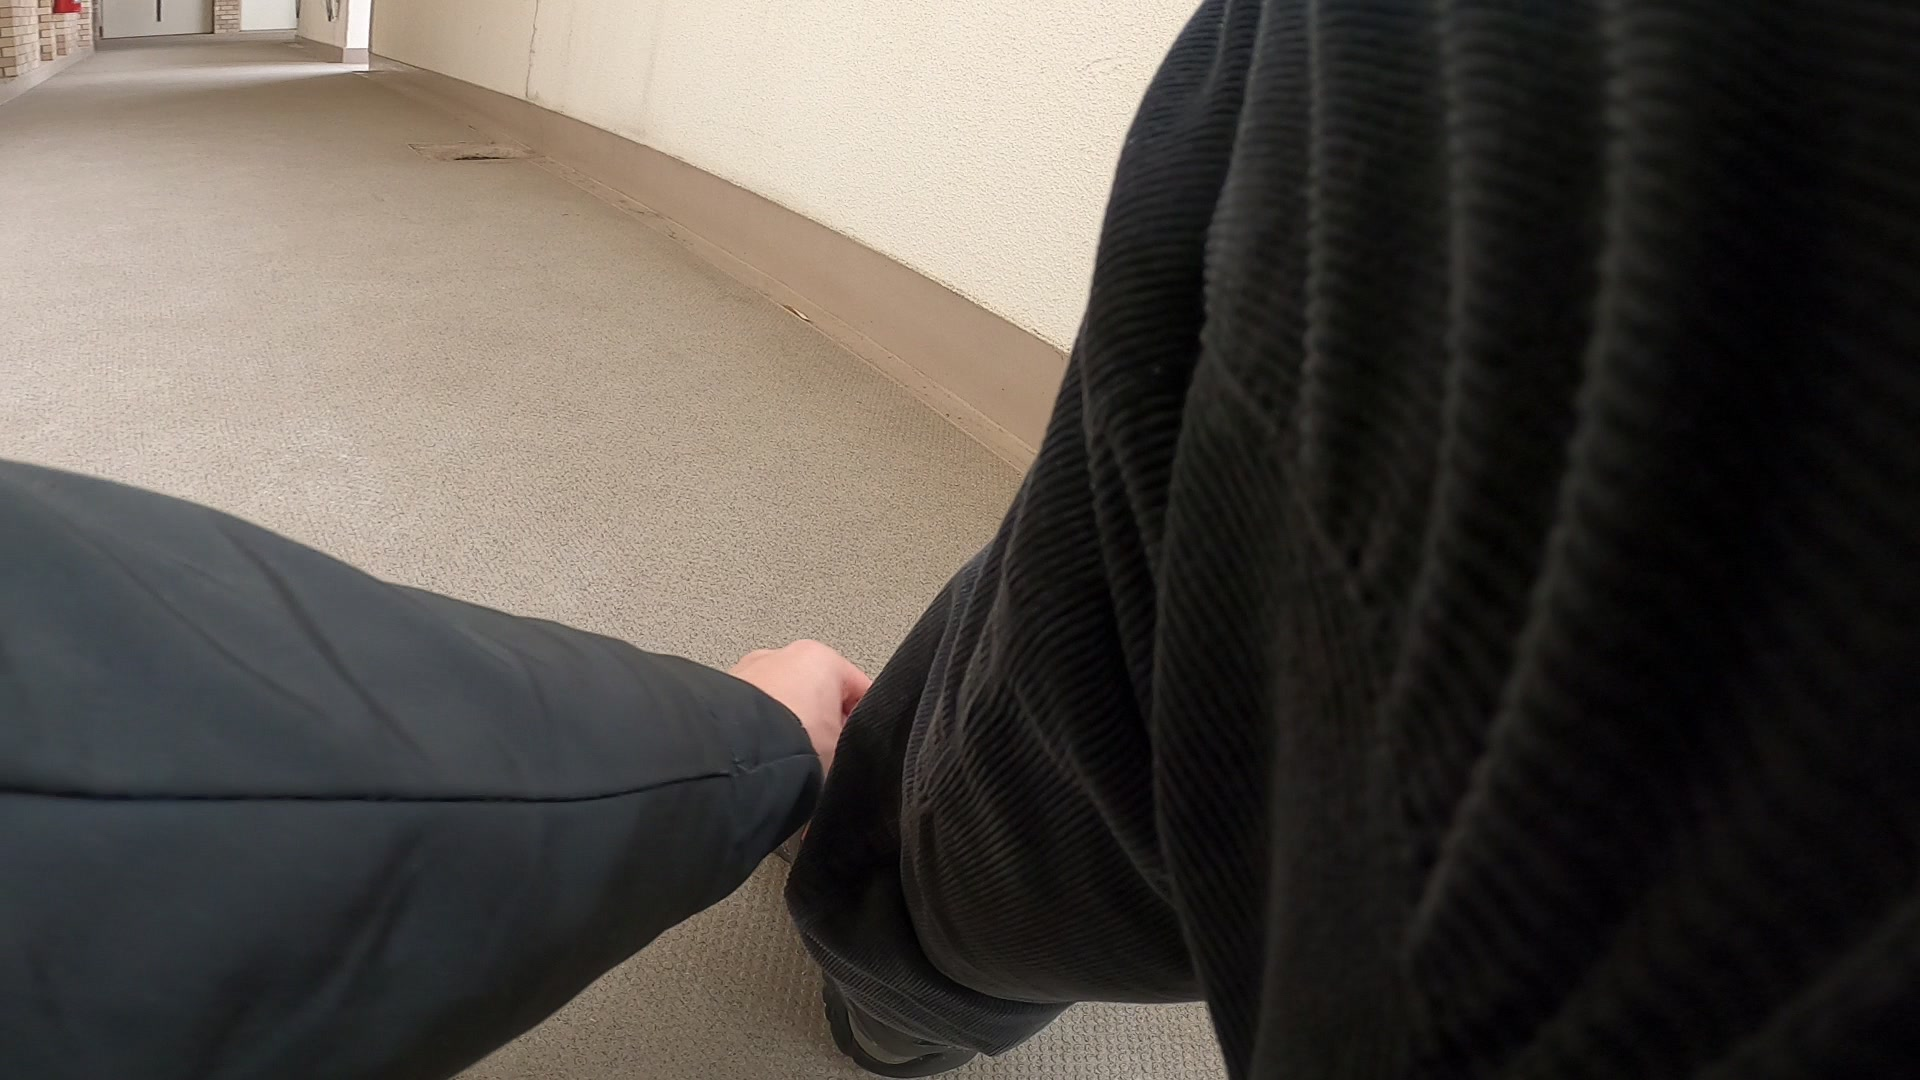
\includegraphics[width=0.75\linewidth]{{thesis/images/temp/6-berth(0.45)}.jpg} 
    \caption*{Berth (45\%)} 
    \vspace{4ex}
  \end{subfigure} 
  \begin{subfigure}[b]{0.5\linewidth}
    \centering
    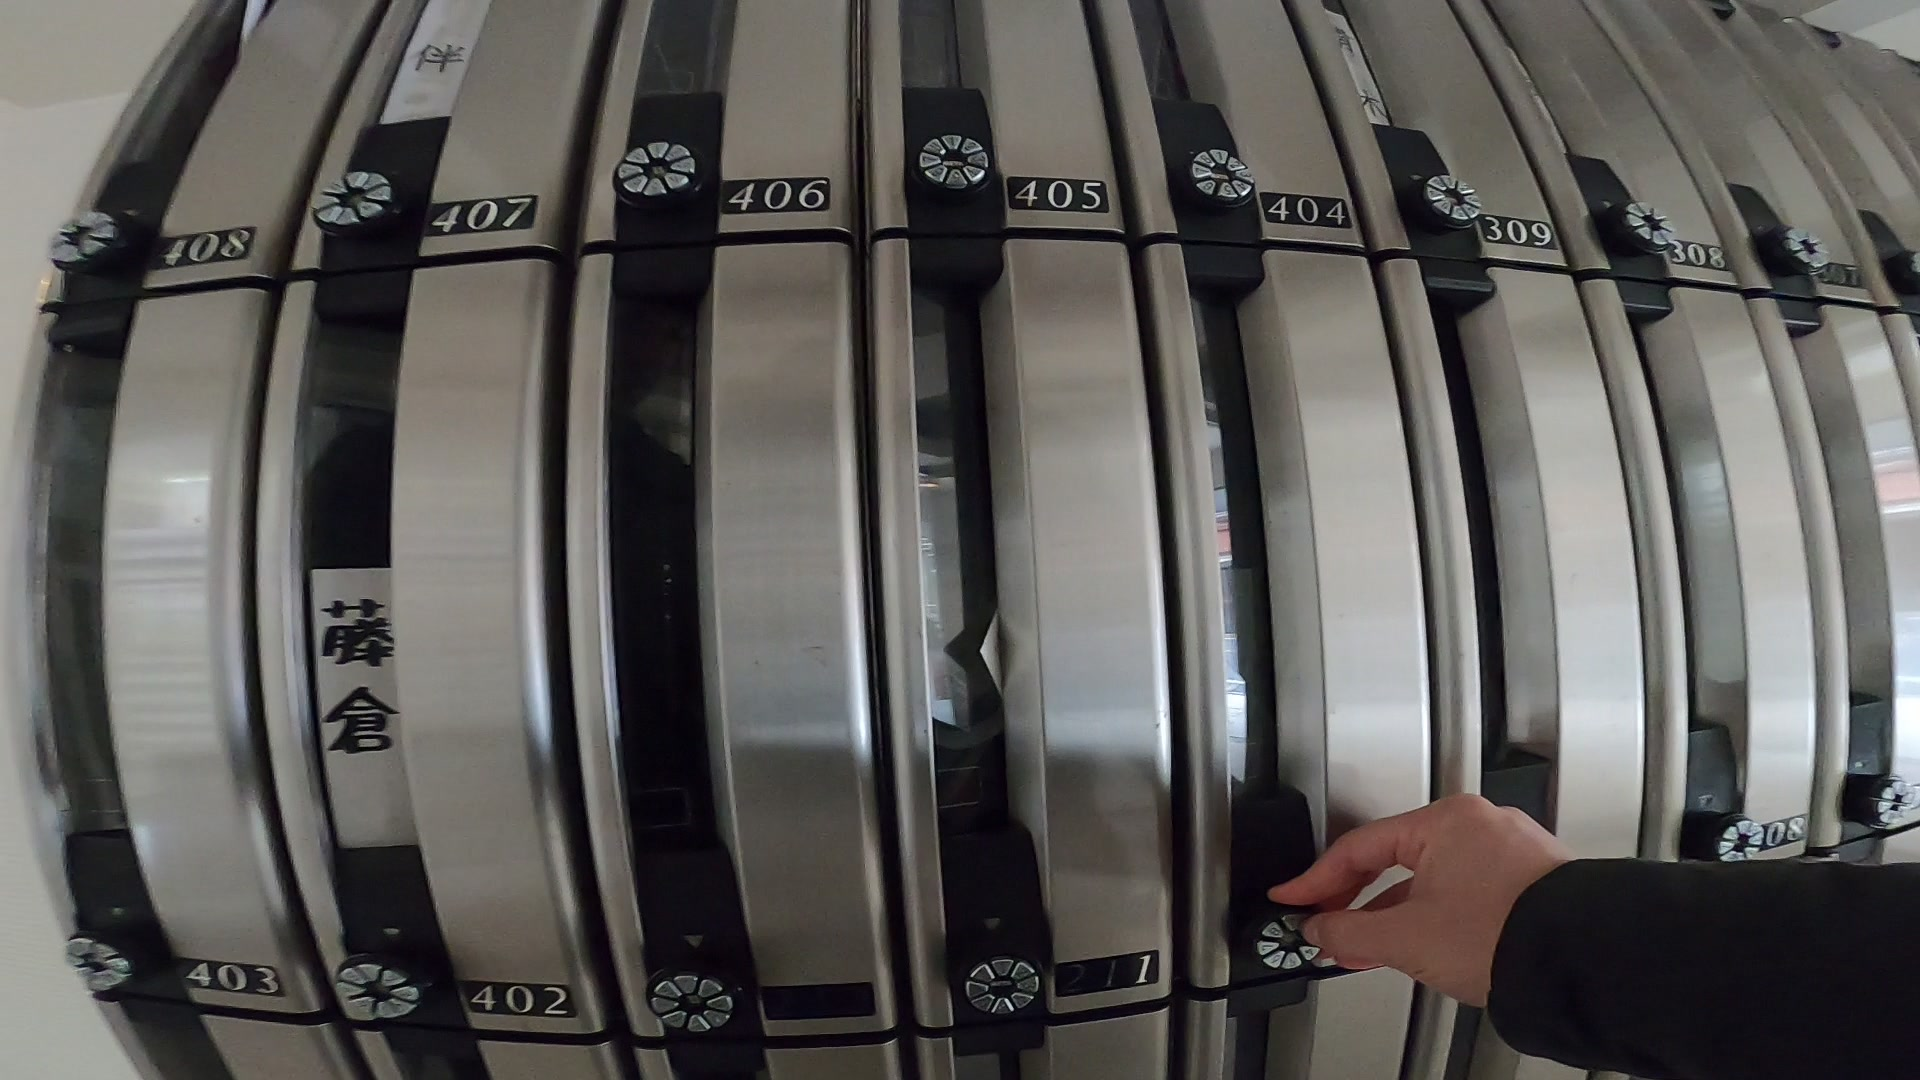
\includegraphics[width=0.75\linewidth]{{thesis/images/temp/7-serverroom(0.25)}.jpg} 
    \caption*{Server Room (25\%)} 
  \end{subfigure}%%
  \begin{subfigure}[b]{0.5\linewidth}
    \centering
    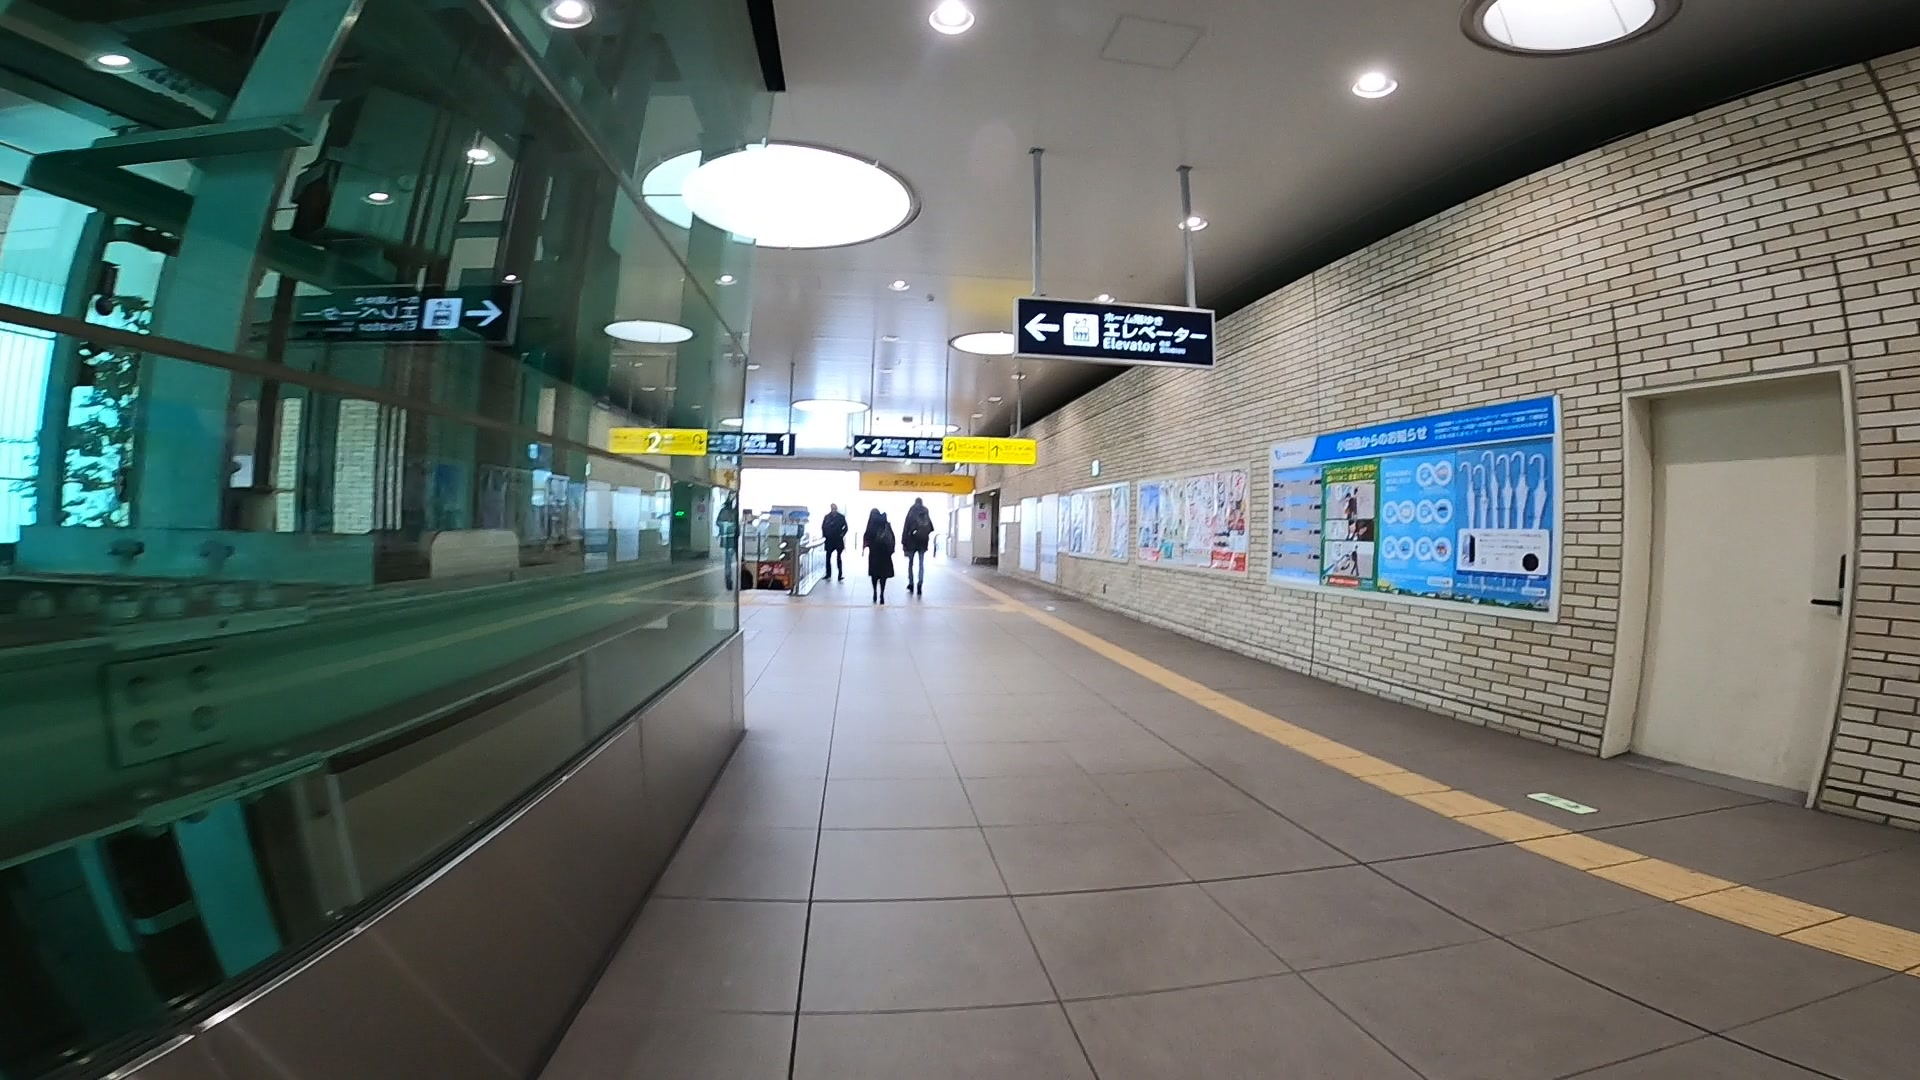
\includegraphics[width=0.75\linewidth]{{thesis/images/temp/9-airportterminal(0.82)}.jpg} 
    \caption*{Airport Terminal (82\%)}
  \end{subfigure} 
  \caption{Illustration of images with wrong classification}
  \label{fig:wrongly} 
\end{figure}



\lhead[\chaptername~\thechapter]{\rightmark}

\rhead[\leftmark]{}

\lfoot[\thepage]{}

\cfoot{}

\rfoot[]{\thepage}

\chapter{Conclusion}
\label{conclusion}

% \begin{paragraph}{Using object re-identification}
% The problem of re-identification \cite{zheng2016person} is an emerging topic in recent years. Although most of the work only deals with person or pedestrians, the idea of re-identification is very suitable for our task of discovering objects of joint attention. During our experiment, we observed that during one specific task, there are certain objects that will attract joint attention multiple times. By adopting the idea of object re-identification, we may be able to find the most relevant object of joint attention, which may be of use for future studies on psychology and group behaviour.
% \end{paragraph}

\section{Summary}

In this thesis, it is demonstrated that efficient models can be obtained by taking advantage of the requirements of each user. 
We applied our idea to both image classification and image retrieval tasks.
In image classification, hierarchical CNN architecture is used to learn the multi-class classification. 
Then, a personalized model, a few branches of the hierarchical CNN, is distributed to each user according to their requirements.
Experiments on CIFAR-10 showed that average users could use a smaller, memory efficient model while maintaining the classification accuracy.
For image retrieval task, our idea is used to reduce the area of the search space to increase the search speed for each user.
By obtaining user requirements in the form of classification labels, each subspace is inspected whether they contain images with any of the user-required labels. 
By finding the relevant sub-spaces and performing the search only on them, a personalized area of search is determined for each user. 
Experimental results revealed that our method works as expected on artificial data whereas it still needs more work to be done for the real-life scenario.

\section{Future Work}

Possible future experiments and the direction of our research will be discussed in the following sections.

\subsection*{Image Classification}

According to our experimental results, each user can obtain a personal, memory-efficient CNN model by using hierarchical CNN.
Although these results are very promising, CIFAR-10 is a relatively small dataset and maintaining the accuracy of the models is not a hard task.
Therefore, the hierarchical CNN method should be tested in a larger dataset to see its true potential. 
However, there are various things to consider before experimenting on a big dataset.

The hierarchy of our model is following a binary tree structure. 
However, there are so many possibilities to construct the hierarchy. 
One example would be a flexible structure, where the branching operation splits the model into 2 or more branches, instead of only 2. 
Even though current experimental results suggest that the accuracy-memory trade-off is better when the depth of the tree is larger, an accuracy drop is expected when the hierarchical model is tested on a bigger dataset.
Furthermore, there is a need to examine alternative hierarchical clustering methods, such as other top-down and bottom-up approaches, to improve memory reduction according to user-required class labels.

The most important future task would be to test our model with real-life user data as user-required classification labels are generated artificially.
One approach of obtaining the real user data would be like the following scheme.
Experiment user group is divided into training and test users. 
We collect egocentric videos of daily activities from the training users.
A set of classification labels are obtained by classifying each user's videos.
These sets of class labels are used to hierarchically cluster the labels to obtain our hierarchy. 
Afterwards, hierarchical CNN with the obtained hierarchy is trained. 
Then, test users are given the whole hierarchical CNN and they start to use it according to our scenario. 
After a fixed time of using the whole model, each user's model is optimized according to the previously classified labels.
The users in the experiment group should be from diverse backgrounds to cover the whole classification labels. 
In this way, an accurate hierarchy can be obtained.


\subsection*{Image Retrieval}

In our experiments, IndexIVFPQ (Inverted File Index + Product Quantization) implementation of FAISS is used as our baseline. 
Current state-of-the-art implementation is IndexIVFPQ used with HNSW (Hierarchical Navigable Small World). 
For our future experiment, we will implement our idea on top of HNSW+IVFPQ to speed up the search according to our idea of reducing the search space according to user requirements.

Experimental results revealed that the results with real-life data are not as good as we expected. 
Possible reasons are discussed in the previous chapter. 
This time, we used videos from the daily-life of only one person for 2 days, first day for training and the other day for testing. 
In the future, longer videos from many users will be used in our experiments.
In order to eliminate the bad training and test frames, a better sampling strategy should be employed.

Places365, a scene recognition dataset, is used in our experiments. 
Because of the existence of many correlated class labels, the accuracy of classifying the labels is relatively low, therefore correctly finding the user-required label is difficult. 
In our future experiments, other datasets can be used to examine our method further. 

We will extend our experiments further to object classification. 
An example scenario will be as the following.
A large object classification dataset, such as ImageNet, will be used to build our search database.
In the training phase of our method, objects seen by the users will be collected to form user-required class labels for each user. 
Afterwards, test users will capture object images from their daily life to search for the most similar objects. 
We hope to examine our method's strengths even more with the object classification task.




\cleardoublepage{}

\lhead[]{Acknowledgments}

\rhead[Acknowledgments]{}


\chapter*{Acknowledgments}

\addcontentsline{toc}{chapter}{Acknowledgments} 




\appendix

\lhead[\chaptername~\thechapter]{\rightmark}

\rhead[\leftmark]{}

\lfoot[\thepage]{}

\cfoot{}

\rfoot[]{\thepage}

\chapter{Additional Results\label{Appen}}


\cleardoublepage{}

\lhead[]{\rightmark}

\rhead[\leftmark]{}

\renewcommand{\bibname}{References}
\bibliographystyle{alpha}
\bibliography{egbib}

\cleardoublepage{}

\lhead[]{Nomenclature}

\rhead[Nomenclature]{}

\printnomenclature[2.5cm]{}
\end{document}
